\documentclass[12pt,twocolumn,tighten]{aastex62}
%\pdfoutput=1 %for arXiv submission
\usepackage{amsmath,amstext,amssymb}
\usepackage[T1]{fontenc}
\usepackage{apjfonts}
\usepackage[figure,figure*]{hypcap}
\usepackage{graphics,graphicx}
\usepackage{hyperref}
\usepackage{comment}

\renewcommand*{\sectionautorefname}{Section} %for \autoref
\renewcommand*{\subsectionautorefname}{Section} %for \autoref

%% Reintroduced the \received and \accepted commands from AASTeX v5.2.
%% Add "Submitted to " argument.
\received{\today}
\revised{---}
\accepted{---}
\submitjournal{AAS journals.}

\shortauthors{Bouma et al.}
\shorttitle{Early Arrival of WASP-4\lowercase{b}}

%\NewPageAfterKeywords

\begin{document}

\title{WASP-4\lowercase{b} Arrived Early for the TESS Mission}

\correspondingauthor{L. G. Bouma}
\email{luke@astro.princeton.edu}

\author[0000-0002-0514-5538]{L. G. Bouma}
\affiliation{ Department of Astrophysical Sciences, Princeton
University, 4 Ivy Lane, Princeton, NJ 08540, USA}
%
\author[0000-0002-4265-047X]{J. N. Winn}
\affiliation{ Department of Astrophysical Sciences, Princeton
University, 4 Ivy Lane, Princeton, NJ 08540, USA}
%
\author[0000-0003-3438-843X]{C. Baxter}
\affiliation{ API, University of Amsterdam, P.O. Box 94249, 1090 GE
    Amsterdam, The Netherlands}
%
\author[0000-0002-0628-0088]{W. Bhatti}
\affiliation{ Department of Astrophysical Sciences, Princeton
University, 4 Ivy Lane, Princeton, NJ 08540, USA}
%
\author[0000-0002-6939-9211]{T. Daylan}
\affiliation{ Department of Physics and Kavli Institute for Astrophysics
and Space Research, Massachusetts Institute of Technology, Cambridge, MA
02139, USA }
%
\author[0000-0002-0875-8401]{J.-M. D\'esert}
\affiliation{ API, University of Amsterdam, P.O. Box 94249, 1090 GE
Amsterdam, The Netherlands}
%
\author[0000-0002-5720-4827]{M. Hill}
\affiliation{Department of Earth Sciences, University of California,
Riverside, CA 92521, USA}
%
\author[0000-0002-7084-0529]{S. Kane}
\affiliation{Department of Earth Sciences, University of California,
Riverside, CA 92521, USA}
%
\author[0000-0002-3481-9052]{K. G. Stassun}
\affiliation{Vanderbilt University, Department of Physics \& Astronomy,
6301 Stevenson Center Lane, Nashville, TN 37235, USA}
\affiliation{Fisk University, Department of Physics, 1000 17th Avenue
N., Nashville, TN 37208, USA}
% 
%-------------------------------------
% TESS Mission Architects:
% These authors should be listed in this order
% see https://spacebook.mit.edu/pages/viewpage.action?pageId=24543276
%-------------------------------------
%
\author{G. R. Ricker} % grr@space.mit.edu WAITING
\affiliation{ Department of Physics and Kavli Institute for Astrophysics
and Space Research, Massachusetts Institute of Technology, Cambridge, MA
02139, USA }
%
\author[0000-0001-6763-6562]{R. Vanderspek} % roland@space.mit.edu WAITING
\affiliation{ Department of Physics and Kavli Institute for Astrophysics
and Space Research, Massachusetts Institute of Technology, Cambridge, MA
02139, USA }
%
\author[0000-0001-9911-7388]{D. W.~Latham} % dlatham@cfa.harvard.edu WAITING
\affiliation{Harvard-Smithsonian Center for Astrophysics, 60 Garden
Street, Cambridge, MA 02138, USA }
%
\author{S. Seager} % seager@mit.edu WAITING
\affiliation{ Department of Earth, Atmospheric, and Planetary Sciences,
Massachusetts Institute of Technology, Cambridge, MA 02139, USA }
%
\author[0000-0002-4715-9460]{J. M.~Jenkins} % jon.jenkins@nasa.gov WAITING
\affiliation{ NASA Ames Research Center, Moffett Field, CA 94035, USA }
%
%-------------------------------------
% 3 representatives of each of SPOC, POC, TSO, for a total of 9. 
%These 9 authors should be listed in alphabetical order
%-------------------------------------
% 3 TSO COAUTHORS
% 3 SPOC COAUTHORS
% 3 POC COAUTHORS
%
\author[0000-0002-3321-4924]{Z. Berta-Thompson} % Zachory.BertaThompson@Colorado.EDU WAITING
\affiliation{Department of Astrophysical and Planetary Sciences,
University of Colorado, Boulder, CO 80309, USA}
%
\author[0000-0003-1963-9616]{D. A. Caldwell} % douglas.Caldwell@nasa.gov % WAITING
\affiliation{ NASA Ames Research Center, Moffett Field, CA 94035, USA }
\affiliation{ SETI Institute, Mountain View, CA 94043, USA}
%
\author[0000-0001-8020-7121]{K. Col\'on} % knicole.colon@nasa.gov WAITING
\affiliation{NASA Goddard Space Flight Center, Exoplanets and Stellar
Astrophysics Laboratory (Code 667), Greenbelt, MD 20771, USA}
%
\author{M. Fausnaugh} % faus@mit.edu WAITING
\affiliation{ Department of Physics and Kavli Institute for Astrophysics
and Space Research, Massachusetts Institute of Technology, Cambridge, MA
02139, USA }
%
\author[0000-0002-5322-2315]{A. Glidden} % aglidden@mit.edu WAITING
\affiliation{ Department of Physics and Kavli Institute for Astrophysics
and Space Research, Massachusetts Institute of Technology, Cambridge, MA
02139, USA }
%
\author{N. Guerrero} % nmg@mit.edu WAITING
\affiliation{ Department of Physics and Kavli Institute for Astrophysics
and Space Research, Massachusetts Institute of Technology, Cambridge, MA
02139, USA }
%
\author[0000-0001-8812-0565]{J. Rodriguez} % rodriguez.jr.joey@gmail.com WAITING
\affiliation{Harvard-Smithsonian Center for Astrophysics, 60 Garden
Street, Cambridge, MA 02138, USA }
%
\author[0000-0002-6778-7552]{J. D. Twicken} % Joseph.Twicken@nasa.gov WAITING
\affiliation{ NASA Ames Research Center, Moffett Field, CA 94035, USA }
\affiliation{ SETI Institute, Mountain View, CA 94043, USA}
%
\author{B. Wohler} % bill.wohler@nasa.gov WAITING
\affiliation{ NASA Ames Research Center, Moffett Field, CA 94035, USA }
\affiliation{ SETI Institute, Mountain View, CA 94043, USA}
%

\begin{abstract}
    The Transiting Exoplanet Survey Satellite (TESS) recently observed
    18 transits of the hot Jupiter WASP-4b.  The sequence of transits
    occurred $81.5 \pm 11.7$~seconds earlier than had been predicted,
    based on earlier data stretching back to 2007.  This is unlikely
    to be the result of a clock error, because TESS observations of
    other hot Jupiters (WASP-6b, 18b, and 46b) are compatible with a
    constant period, ruling out an 81.5-second offset at the
    6.4$\sigma$ level.  The 1.3-day orbital period of WASP-4b appears
    to be decreasing at a rate of $\dot{P} = -12.6 \pm 1.2$
    milliseconds per year.  This might be caused by tidal orbital
    decay or apsidal precession, although both interpretations have
    shortcomings.  The gravitational influence of a third body is another
    possibility, although at present there is scant evidence for such a
    body. Further observations are needed to confirm and
    understand the timing variation.
\end{abstract}

\keywords{
  planet-star interactions ---
  planets and satellites: individual (WASP-4b, WASP-5b, WASP-6b,
    WASP-12b, WASP-18b, WASP-46b) ---
  binaries: close
}


%%%%%%%%%%%%%%%%%%%%%%%%%%%%%%%%%%%%%%%%%%
\section{Introduction}
\label{sec:intro}

Although the Transiting Exoplanet Survey Satellite (TESS) is designed
to detect new planets, it will also perform precise photometric
monitoring of most of the planets that have been discovered by
ground-based transit surveys over the last two decades.  One of the
applications of the new TESS data is to search for timing anomalies in
hot Jupiter systems.  Long-term monitoring of hot Jupiter transit and
occultation times should eventually reveal two distinct processes.

First, whenever the orbital angular momentum is less than 3 times the
rotational angular momentum, the system is vulnerable to tidal orbital
decay \citep{counselman_outcomes_1973,hut_stability_1980}.  Most hot
Jupiters satisfy this condition and their orbits should be shrinking
\citep{levrard_falling_2009,matsumura_tidal_2010}.  The rate of decay,
which depends on how friction dissipates the energy of tidal
disturbances, is difficult to observe directly or calculate from first
principles. This has been a stubborn source of uncertainty in the
interpretation of many phenomena in stellar and planetary astrophysics
(as reviewed by \citealt{Mazeh2008} and \citealt{ogilvie_tidal_2014}).

Second, long-term timing studies may reveal apsidal precession, {\it
  i.e.}, the rotation of the orbital ellipse within the orbital
plane. Apsidal precession has long been observed in eclipsing binaries
\citep[{\it e.g.},][]{
  schwarzschild_structure_1958,torres_accurate_2010,borkovits_eclipse_2015}.
For exoplanets, precessing orbits have been detected in a handful of
cases, including circumbinary systems (Kepler-413
\citealt{kostov_kepler-413b_2014}; Kepler-453
\citealt{welsh_kepler_2015}, planets orbiting rapidly rotating stars
(Kepler-13
\citealt{szabo_spin-orbit_2012,szabo_mapping_2014},~\citealt{masuda_spin-orbit_2015};
and systems with multiple interacting giant planets (Kepler-108
\citealt{mills_kepler-108_2017}; Kepler-693
\citealt{masuda_eccentric_2017}).  Apsidal precession is not regularly
observed in hot Jupiter systems because their orbits are nearly
circular, which may itself be a consequence of star-planet tides.  If
it could be observed, then \citep{ragozzine_probing_2009} showed that
it would be possible to measure the planet's Love number, which would
be a valuable constraint on the planet's interior.

So far, the most convincing direct evidence for either orbital decay
or apsidal precession has come from WASP-12b.
\citet{maciejewski_departure_2016} and \citet{patra_2017} showed that
the transit period of WASP-12b has been steadily decreasing by about
30~milliseconds per year over the last decade.  Here, we present
evidence for a timing anomaly in the WASP-4 system.  The hot Jupiter
WASP-4b orbits a G7V star every 1.34 days, corresponding to an orbital
distance of 5.5 stellar radii
\citep{wilson_wasp-4b_2008,hoyer_tramos_2013}.  It is a good target to
search for departures from a constant period, because transit data
exists all the way back to 2007.  The orbital eccentricity is less
than 0.018 (2$\sigma$), based on the work of
\cite{knutson_friends_2014}, who combined the available transit times,
occultation times, and Doppler data.  The stellar obliquity (or at
least its sky projection) is also compatible with zero, within about
10 degrees
\citep{triaud_spin-orbit_2010,beerer_secondary_2011,sanchis-ojeda_starspots_2011}.

In what follows, \S~\ref{sec:observations} presents the new TESS
observations, and \S~\ref{sec:timing} describes our timing
analysis.  We tried fitting the data with three models: a constant
period, a decaying period, and a slightly eccentric precessing orbit.
A constant period can be ruled out, but we cannot distinguish between
the latter two possibilities.  Either possibility would have
interesting implications, described in \S~\ref{sec:implications}.
Appendix~\ref{sec:verify_tess} considers the possibility that the
WASP-4 timing anomaly is due to an error in time stamps in the TESS
data products.  We found this possibility to be unlikely because none
of the other hot Jupiters we examined show a timing offset with the
same amplitude as was seen for WASP-4.


%%%%%%%%%%%%%%%%%%%%%%%%%%%%%%%%%%%%%%%%%%
\section{New transits and system parameters}
\label{sec:observations}

\begin{figure}[t]
    \begin{center}
        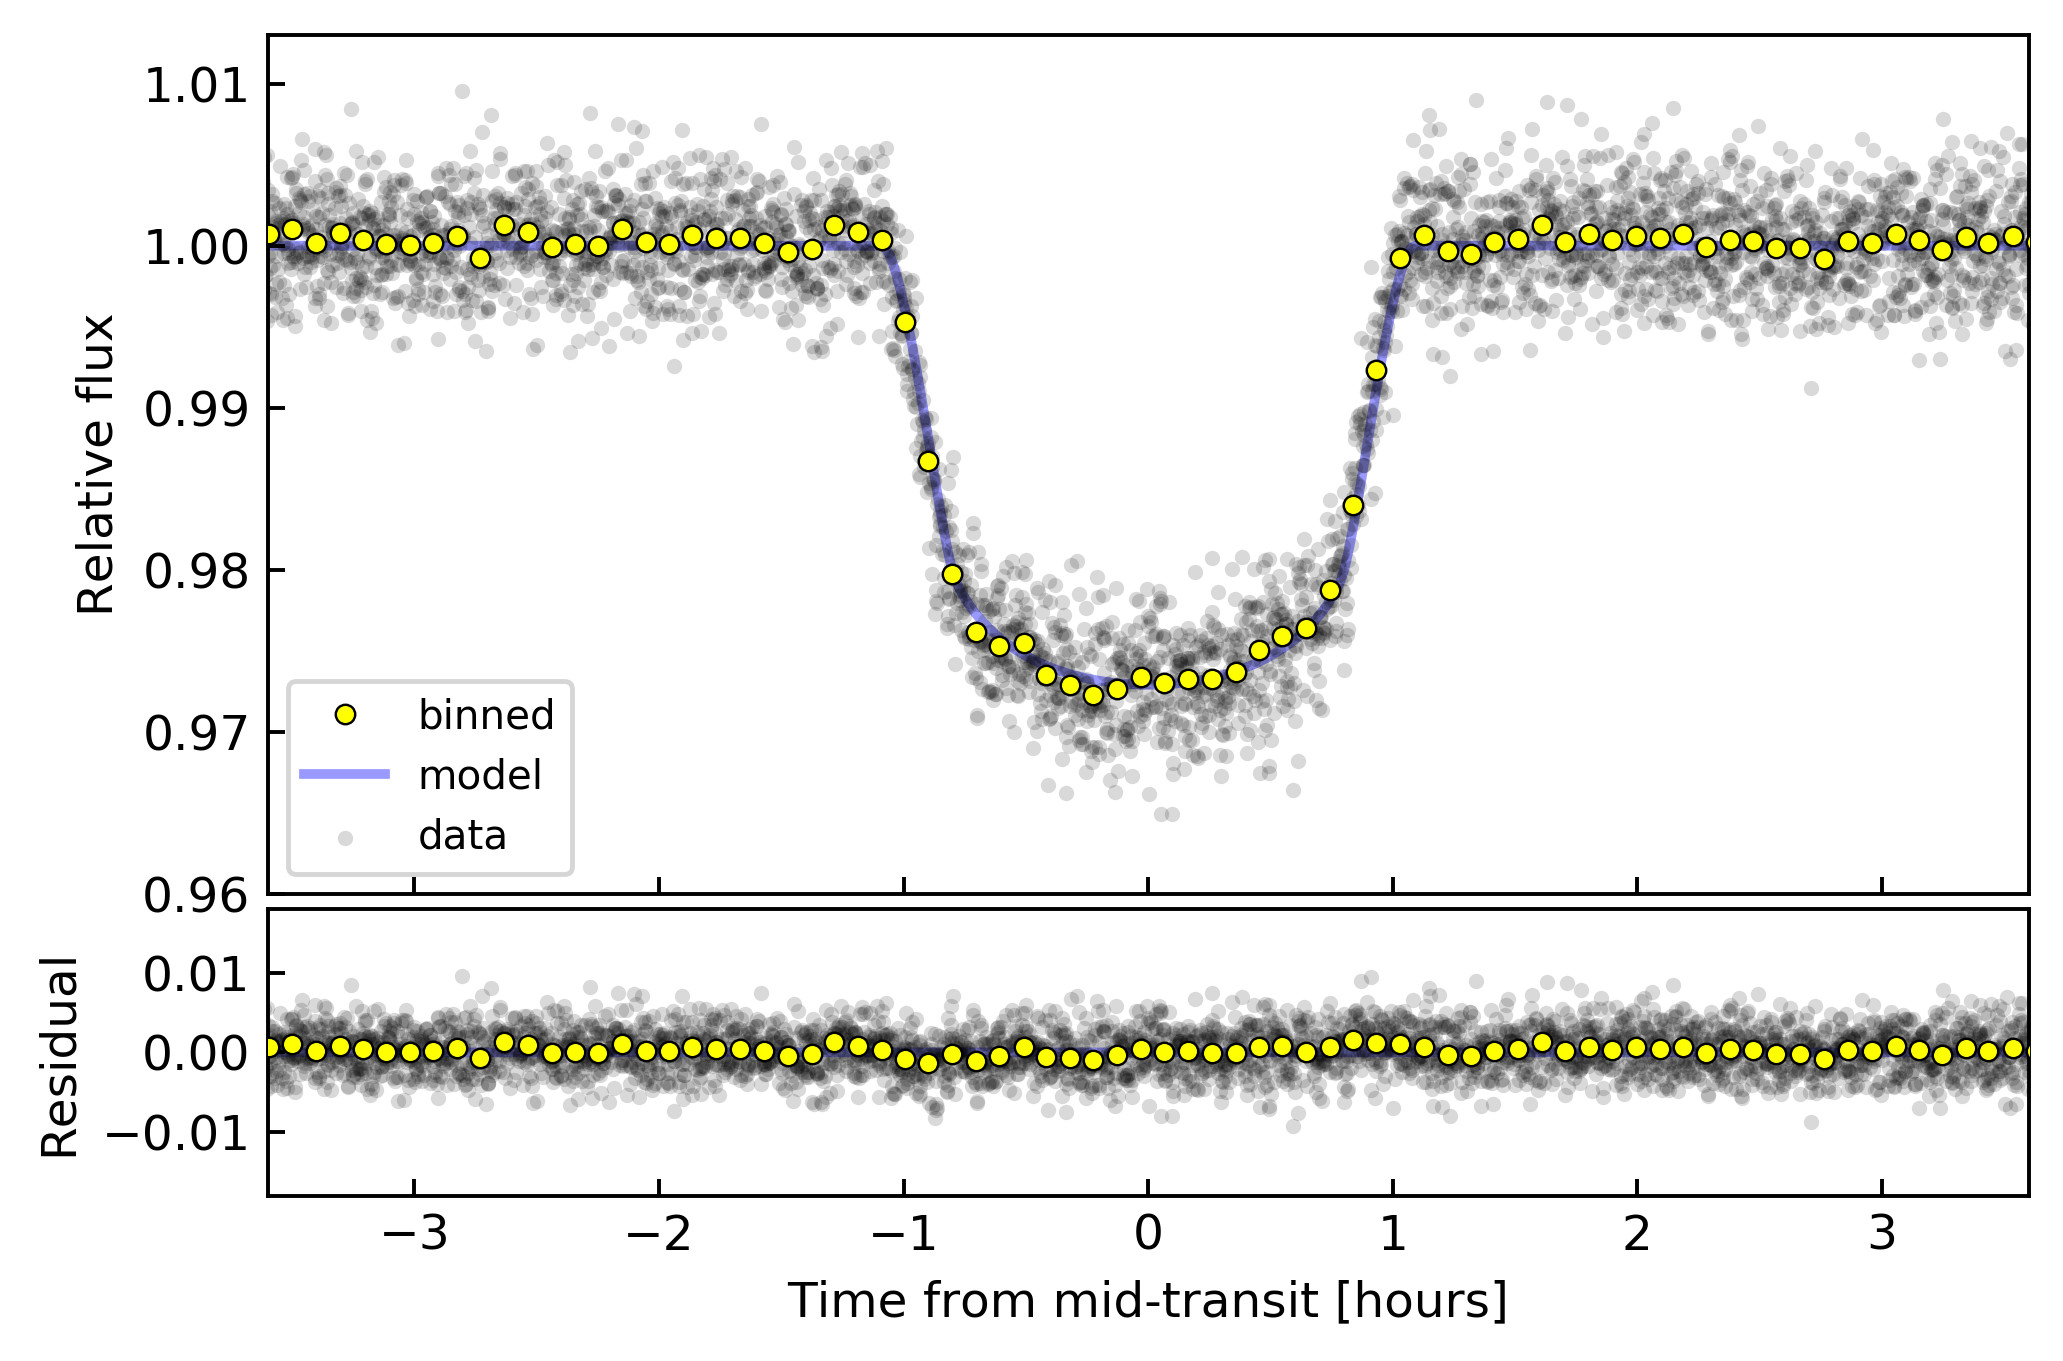
\includegraphics[width=0.49\textwidth]{f1.png}
    \end{center}
    \vspace{-0.5cm}
    \caption{
      {\bf TESS observations of WASP-4b.} On the left, black points
      are TESS flux measurements, with a vertical offset applied. Blue
      curves are best-fit models. The numbers printed next to each
      lightcurve are the approximate transit times expressed in
      BJD minus 2{,}457{,}000.  The right side shows the
      residuals.
       \label{fig:lightcurves}
    }
\end{figure}

\begin{figure}[t]
    \begin{center}
        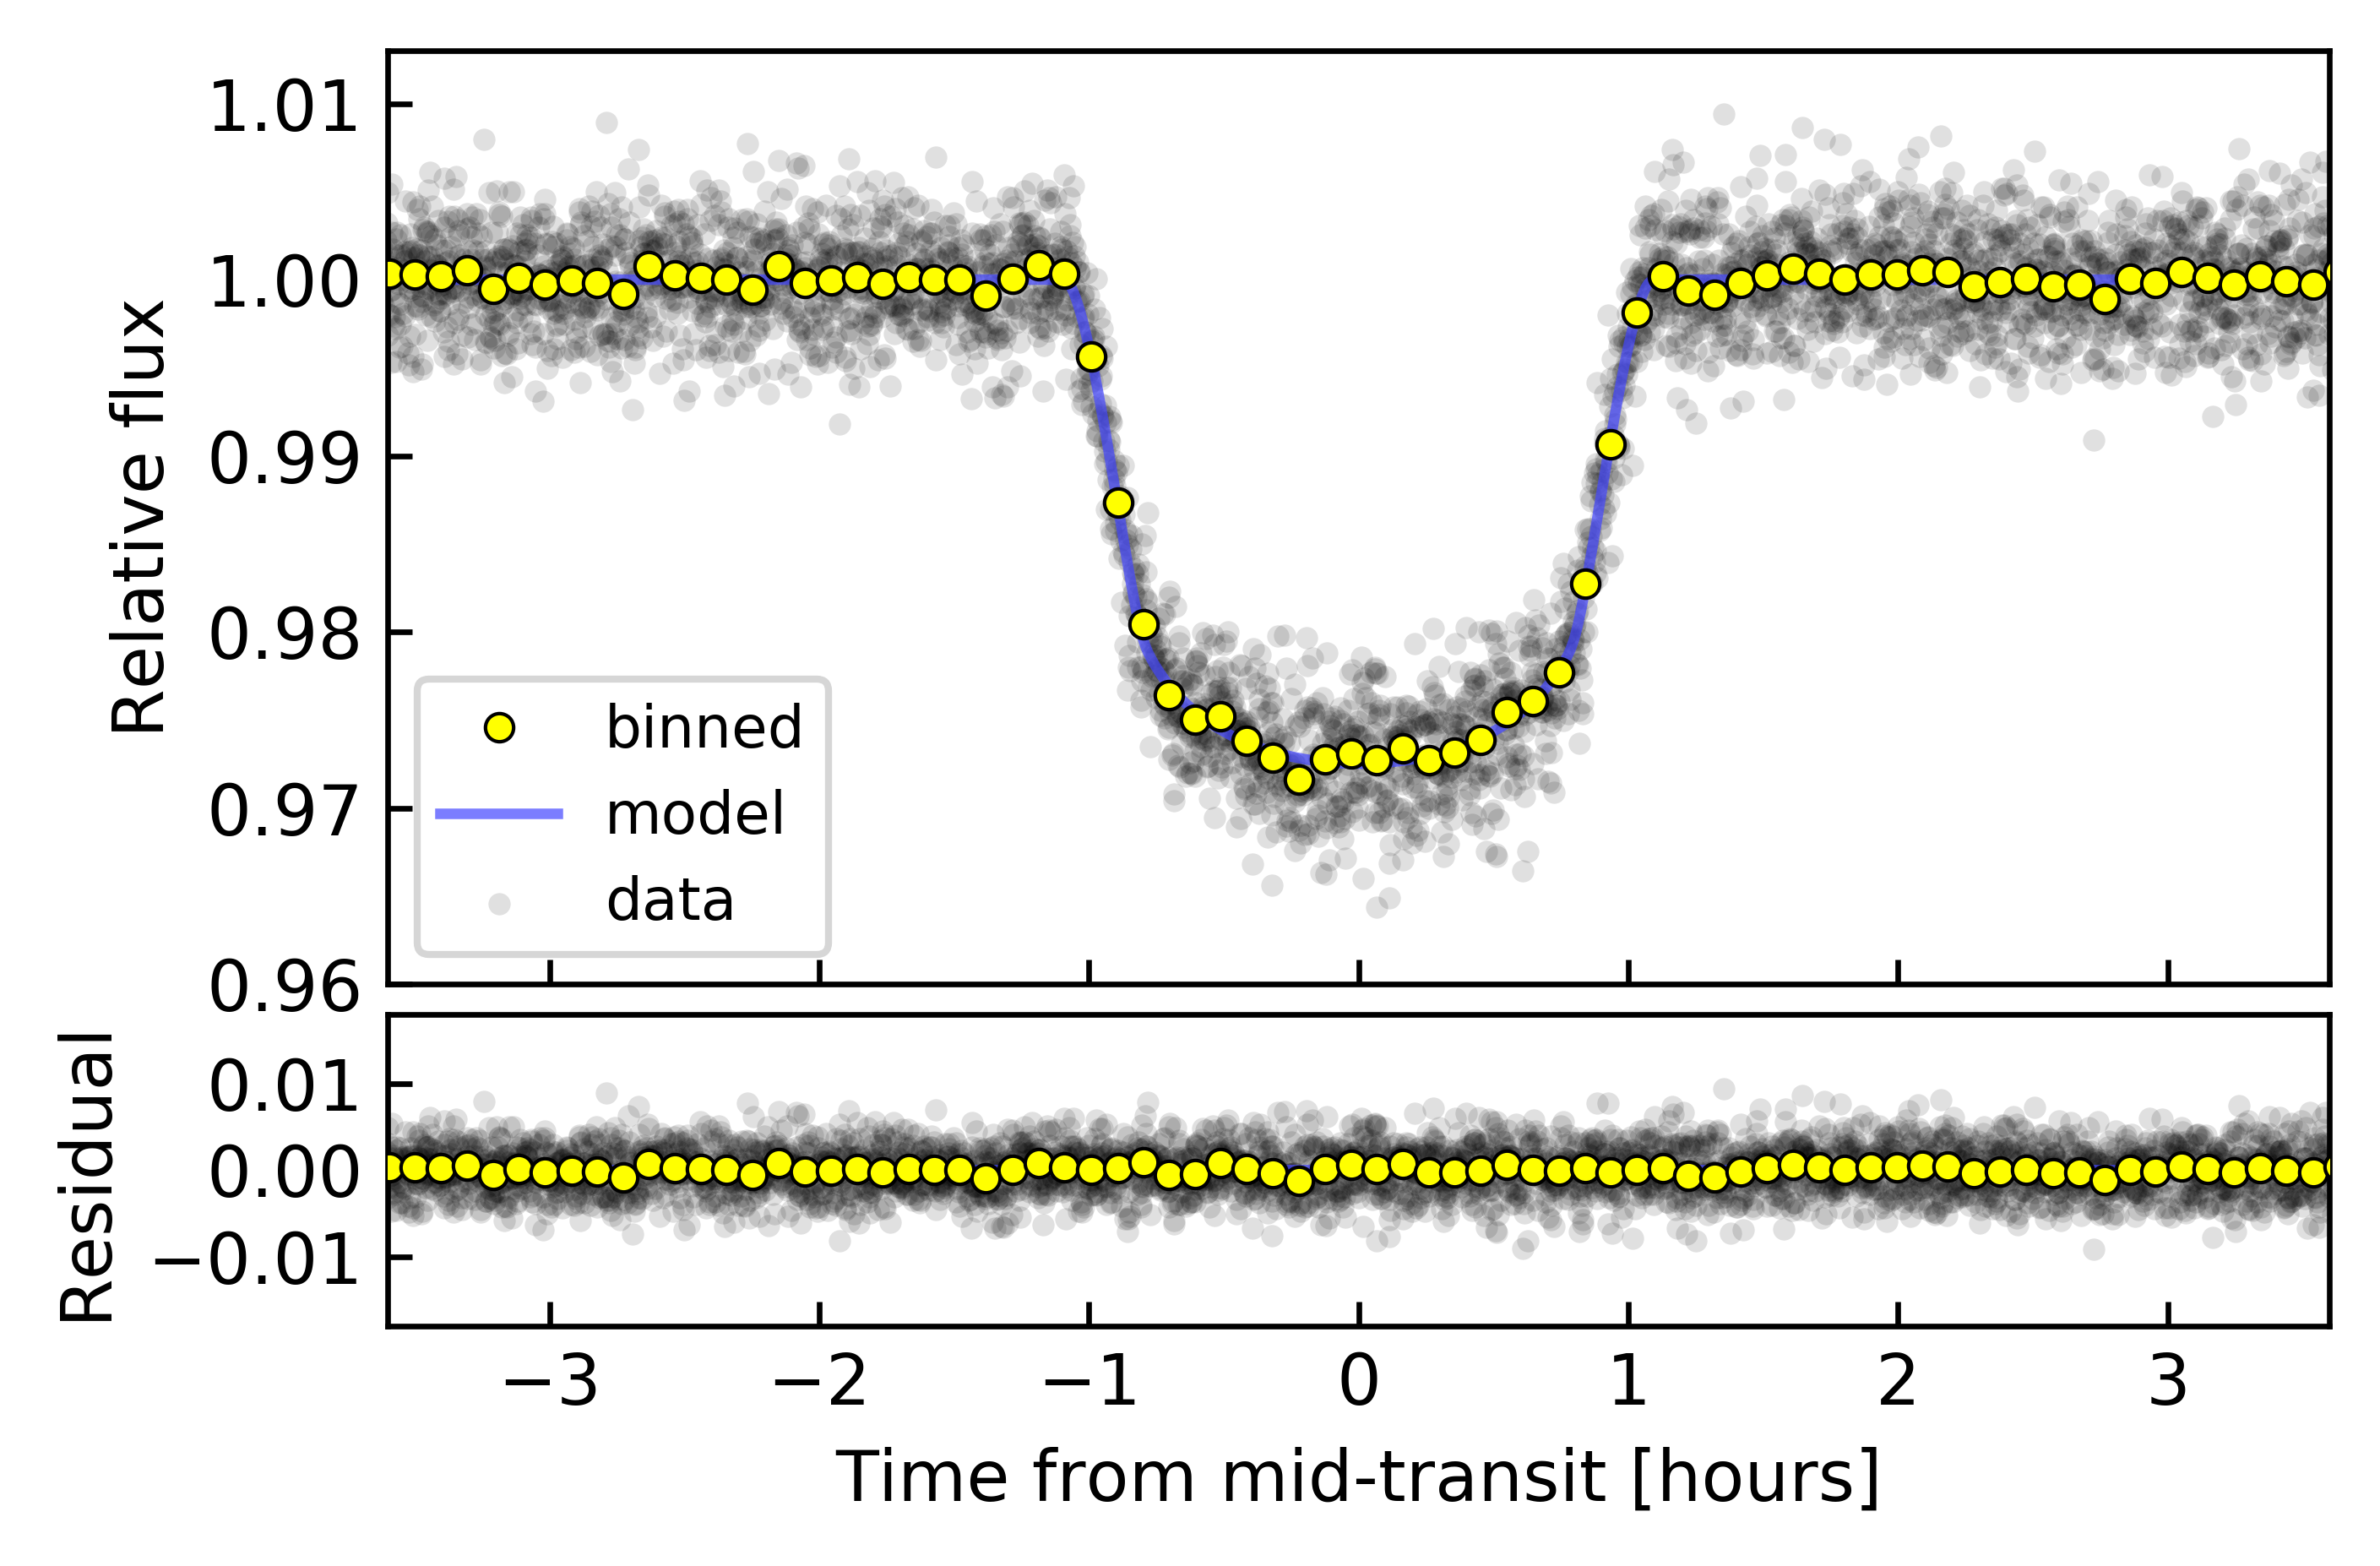
\includegraphics[width=0.49\textwidth]{f2.png}
    \end{center}
    \vspace{-0.5cm}
    \caption{
        {\bf Phase-folded lightcurve of WASP-4b.} Black points are
        TESS data. Yellow points are binned measurements.  The bottom
        panel shows the residuals.  The fit to the phase-folded
        transit (blue line) is used when measuring mid-transit times for
        the individual transits (Figure~\ref{fig:lightcurves}).
        \label{fig:phasefold}
    }
\end{figure}

\subsection{Observations}

WASP-4 was observed by TESS with Camera 2 from August 23 to September
20, 2018, within the second ``sector'' of science operations.  The
star is designated as TIC 402026209 in the TESS Input Catalog
\citep{stassun_TIC_2018}.  The pixel data for an $11\times11$ array
surrounding WASP-4 were averaged into 2-minute stacks by the onboard
computer.  The data were downlinked via the Deep Space Network. The
timestamps from the spacecraft clock were then transformed by the
Payload Operations Center into the {\it Temps Dynamique Barycentrique}
(TDB) reference system.  The images were then reduced to lightcurves
by the Science Processing Operations Center (SPOC) at NASA
Ames~\citep{jenkins_tess_2016}.  During this processing, the SPOC used
the known spacecraft trajectory to compute the barycentric time
corrections on a target by target basis, and expressed the timestamps
as Barycentric TESS Julian Dates (BTJD), which is simply the
barycentric Julian date minus 2{,}457{,}000.  The lightcurves were
vetted and released by the MIT TESS Science Office to the Mikulski
Archive for Space Telescopes on November 29,
2018~\citep{ricker_tess_alerts_2018}.

We began our analysis with the Presearch Data Conditioning (PDC)
lightcurve \citep{smith_kepler_apertures_2017,smith_kepler_PDC_2017}.
We processed the lightcurve as follows.  First, we removed all points
with non-zero quality flags.  This removed data contaminated by coarse
spacecraft pointing, cosmic rays, and other annoyances
\citep{tess_data_product_description_2018}.  We also removed the data
within the first and last hours of both orbits, because of ramp-like
systematic effects that appear during those time ranges. We also
removed the data that might have been adversely affected by ``momentum
dumps,'' the firing of thrusters and resetting of reaction wheels that
took place every 2.5 days during sector
2.\footnote{\url{archive.stsci.edu/hlsps/tess-data-alerts/hlsp_tess-data-alerts_tess_phot_s01_tess_v1_release-notes.pdf}}.
The data during these events were assigned quality flags corresponding
to ``Reaction Wheel Desaturation Event'' and ``Manual Exclude''.  For
WASP-4, these flags were simultaneously set for 54 distinct cadences,
and there were 10 momentum dumps, averaging about 10 minutes of
flagged data per dump.  Out of caution, we clipped out an additional
10 minutes before and after every momentum dump.

All told, we removed 8\% of the original data points, and were left
with 18{,}165 measurements of the relative flux of WASP-4.  We
normalized the data by dividing out the median flux.  We converted the
timestamps from BTJD into BJD by adding the appropriate 2457000 day
offset \citep{tess_data_product_description_2018}.  Many of these and
subsequent processing steps were performed using
\texttt{astrobase}~\citep{bhatti_astrobase_2018}. We did not
``flatten'' the lightcurves, as is often done with splines,
polynomials, or Gaussian processes.  Instead, we modeled the
out-of-transit flux variations simultaneously with the transit parameters,
as described below.

\subsection{Measuring the transit times}
\label{sec:measurement}

Using the cleaned PDC lightcurve, we used the Box Least Squares
algorithm \citep{kovacs_box-fitting_2002} to estimate the orbital
period, transit duration, and a reference epoch using the TESS data
alone.  Based on the results, we isolated the data within 4 transit
durations of each transit midpoint.  We then fitted all of the transit
data using the analytic formulae given by \citet{mandel_analytic_2002}
and implemented by \citet{kreidberg_batman_2015}.  We assumed the
orbit to be circular. The free parameters were the reference epoch,
the planet to star radius ratio $R_{\rm p}/R_\star$, the orbital
distance to stellar radius ratio $a/R_\star$, the inclination $i$, two
quadratic limb-darkening coefficients $(u_{\rm linear}, u_{\rm
  quad})$, and the orbital period $P$.

We sampled the posterior probability distribution for all the
parameters using the algorithm proposed by
\citet{goodman_ensemble_2010} and implemented by
\citet{foreman-mackey_emcee_2013}.  Table~1 gives the results, which
are in reasonable agreement with the parameters reported by {\it
  e.g.}, \citet{southworth_high-precision_2009} and
\citet{huitson_gemini_2017}.  Figure~\ref{fig:phasefold} shows the
phase-folded lightcurve.

To measure the transit times, we fitted each transit separately, with
four free parameters: the time of mid-transit $t_{\rm tra}$, the
planet-to-star radius ratio, and the slope and intercept of a linear
trend to account for any slow variations unrelated to the transit.  We
fixed the remaining parameters at the values that had been determined
from the phase-folded TESS lightcurve.  The uncertainty in each
data point was set equal to the root-mean-square (rms) level of the
out-of-transit data.

To verify that the measured uncertainties are plausible, we computed
the reduced $\chi^2$ for a linear ephemeris fit to the measured TESS
transit times.  We found that $\chi^2 = 9.2$, with $n=16$ degrees of
freedom.  The variance of the $\chi^2$ distribution is $2n$, so we
would expect $\chi^2 16 \pm 5.7$.  Visually inspecting the residuals
showed that the error variance had been overestimated, so we
multiplied the measured TESS errors by a factor $f=0.76$, forcing a
reduced $\chi^2$ of unity.  This lowered the mean uncertainty of the
transit midtimes from $29.8$ to $22.6$ seconds.  We verified that
omitting this step did not appreciably alter any of our conclusions.

Figure~\ref{fig:lightcurves} shows the lightcurve of each transit, the
best-fit models, and the residuals.  Table~2 reports the mid-transit
times and their uncertainties.  After binning the residuals to 1-hour
windows, the lightcurves have an rms scatter of 586\,{\rm ppm}.  The
pre-launch TESS noise model\footnote{\url{github.com/lgbouma/tnm}} \citep{winn_photonflux_2013,Sullivan_2015}
would have predicted an error
budget consisting of the following terms added in quadrature:
410\,{\rm ppm} from photon-counting noise, 202\,{\rm ppm} from
detector read noise, and 673\,{\rm ppm} from the zodiacal background
light.  The level of background light appears to have been
overestimated.

\subsection{Star and planet parameters}
\label{sec:system_parameters}

\begin{deluxetable}{lccc}
\tabletypesize{\scriptsize}
\tablecaption{Selected system parameters of WASP-4b\label{tbl:params}}
\tablenum{1}

\tablehead{
\colhead{Parameter} & \colhead{Value} & \colhead{68\% Confidence Interval} & \colhead{Comment}
}

\startdata
{\it Transit/RV parameters:} & & & \\
  $R_{\rm p}/R_\star$                        & $0.15117$              & $+0.00047$, $-0.00037$      & A \\
  $i$~[deg]                                  & $88.85$                & $+0.77$, $-0.90$            & A \\
  $a/R_\star$                                & $5.457$                & $+0.030$, $-0.066$          & A \\
  $u_{\rm linear}$                           & $0.388$                & ---                         & A \\
  $u_{\rm quad}$                             & $0.212$                & ---                         & A \\
  $K$~[m~s$^{-1}$]                           & $241.1$                & $+2.8$, $-3.1$              & B \\
{\it Stellar parameters:} & & & \\
  $T_{\rm eff}$~[K]                          & $5400$                 & $\pm 90$                    & C \\
  $\log g_\star$~[cgs]                       & $4.47$                 & $\pm 0.11$                  & C \\
  $[{\rm Fe/H}]$                             & $-0.07$                & $\pm 0.19$                  & C \\
  $F_{\rm bol}$~[erg~cm$^{-2}$~s$^{-1}$]     & $2.802\times10^{-10}$  & $\pm 0.076\times10^{-10}$   & D \\
  $\pi$~[mas]                                & $3.7145$               & $0.0517$                    & F \\
  $R_\star$~[R$_{\odot}$]                    & $0.893$                & $\pm 0.034$                 & E \\
  $\rho_\star$~[g~cm$^{-3}$]                 & $1.717$                & $+0.029$, $-0.062$          & E \\
  $M_\star$~[M$_{\odot}$]                    & $0.867$                & $+0.087$, $-0.097$          & E \\
  $T$ magnitude                              & $11.778$               & $\pm 0.018$                 & G \\
{\it Planetary parameters:} & & & \\
  $a$~[AU]                                   & $0.0227$               & $\pm 0.0008$                & E \\
  $M_p$~[M$_{\rm Jup}$]                      & $1.189$                & $+0.093$, $-0.104$          & E \\
  $R_p$~[R$_{\rm Jup}$]                      & $1.314$                & $\pm 0.039$                 & E \\
\enddata

\tablecomments{
  (A) From phase-folded TESS lightcurve (\S~\ref{sec:measurement}).
  Orbital periods are in Table~4. The limb darkening parameters were
  allowed to float around the \citet{claret_limb_2017} prediction, but
  were unconstrained.
  (B) \citet{triaud_spin-orbit_2010}.
  (C) From HARPS spectra \citep{doyle_accurate_2013}.
  (D) \citet{stassun_accurate_2017}.
  (E) From functions of stellar, transit or RV parameters as discussed in text.
  (F) \citet{gaia_collaboration_gaia_2018}.
  (G) \citet{stassun_TIC_2018}.
}

\end{deluxetable}

We calculated the stellar and planetary parameters in the following
way.  We computed the star's spectral energy distribution based on the
{\it Gaia} DR2 parallax (after making the small correction advocated
by \citealt{stassun_evidence_2018}) and the broadband magnitudes from
all the available all-sky catalogs: $G$ from {\it Gaia\/} DR2, $B_T$
and $V_T$ from {\it Tycho-2}, $BVgri$ from {\it APASS}, $JHK_S$ from
{\it 2MASS}, and the {\it WISE}~1--4 passbands, thus spanning the
wavelength range 0.4--22~$\mu$m.  We adopted the effective temperature
from the work by \citet{doyle_accurate_2013}, who determined the
spectroscopic parameters of WASP-4 using high-signal-to-noise
observations with the High Accuracy Radial-velocity Planet Searcher
(HARPS).  Then, we determined the stellar radius through the
combination of the bolometric luminosity and the effective
temperature, using the Stefan-Boltzmann law.  To determine the stellar
mass, we first computed the mean stellar density based on the value of
$a/R_\star$ that gave the best fit to the phase-folded TESS lightcurve
(for the relevant equation, see \citealt{seager_unique_2003} or
\citealt{winn_exoplanet_2010}).  The mass was calculated from the
radius and density, and the orbital distance was also calculated from
the radius and $a/R_\star$.  The planetary radius was calculated as
the product of $R_\star$ and $R_{\rm p}/R_\star$.  Finally, the planet
mass was calculated based on the stellar mass, the radial-velocity
amplitude observed by \citet{triaud_spin-orbit_2010}, and the orbital
inclination.

Table~1 gives the resulting parameters, which we adopted for the
remaining analysis.  Our parameters are in agreement with those of
previous investigators
\citep{wilson_wasp-4b_2008,gillon_discovery_2009,winn_transit_2009,southworth_homogeneous_2011,petrucci_no_2013}.
By comparing the star's luminosity and spectroscopic parameters with
the outputs of the Yonsei-Yale stellar-evolutionary models, we found
that WASP-4 is a main-sequence star with an age of approximately
$7\,{\rm Gyr}$.


%%%%%%%%%%%%%%%%%%%%%%%%%%%%%%%%%%%%%%%%%%
\section{Timing analysis}
\label{sec:timing}

\begin{figure}[t]
    \begin{center}
        \leavevmode
        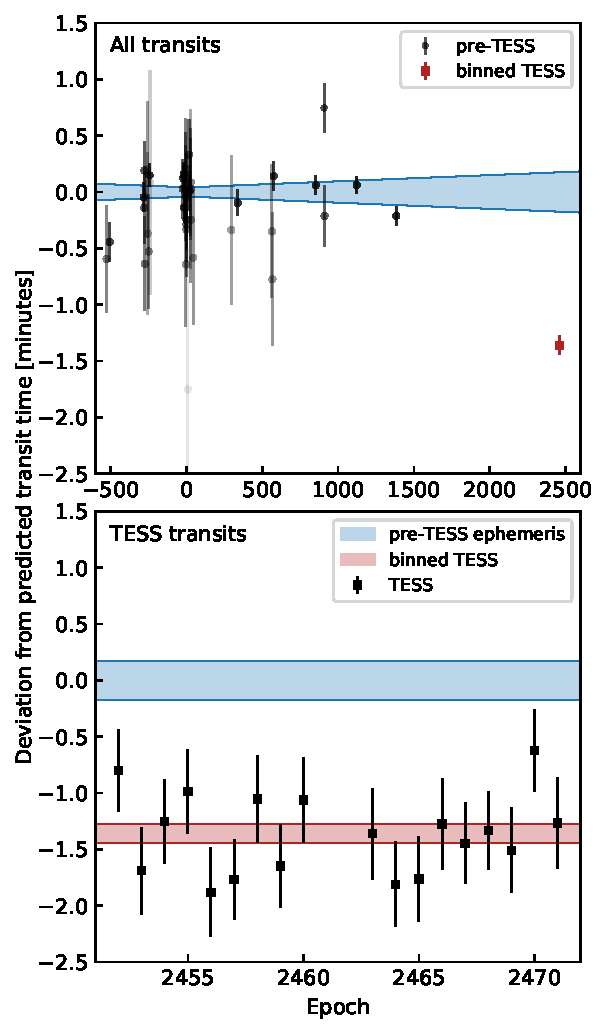
\includegraphics[width=0.49\textwidth]{f3.pdf}
    \end{center}
    \vspace{-0.6cm}
    \caption{ {\bf TESS saw WASP-4b transit earlier than expected.}
      Both plots show the deviations between the observed and
      calculated transit times, where the calculation is based only on
      the pre-TESS data and assumes a constant period.  The blue bands
      depict the $\pm$$1\sigma$ credible interval of the predicted
      times.  {\it Top:} The full timing dataset spans 10 years. The
      darkest points correspond to the most precise data.  {\it
        Bottom:} Close-up of the TESS observations. The red band shows
      the average deviation of the TESS data, which is $81.5 \pm
      11.7\ {\rm seconds}$.
        \label{fig:arrived_early}
    }
\end{figure}

\begin{figure*}[t]
	\begin{center}
		\leavevmode
		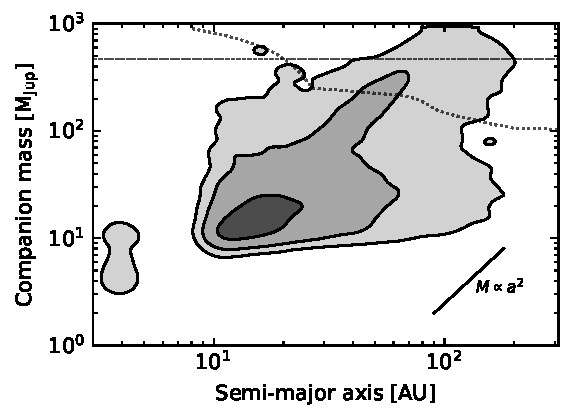
\includegraphics[width=0.9\textwidth]{f4.pdf}
	\end{center}
	\vspace{-0.5cm}
	\caption{ {\bf Timing residuals and best-fit models for WASP-4b.}
		The residuals are the observed times minus the calculated times
		assuming a constant period.  The darkest points correspond to
		the most precise data. The constant-period model (gray line) is
		a poor description of the data.  Models with a uniformly
		decreasing period (blue) or apsidal precession (orange) provide
		better fits to the data.  The red square represents the
		combination of all the TESS data and is for display purposes
		only.  The models were fitted to all of the individual transit
		times.
		\label{fig:times}
	}
\end{figure*}


\subsection{Pre-TESS timing measurements}
\label{subsec:times}

Table~2 gives the transit times we used in our analysis. We included
data from peer-reviewed literature for which the analysis was based on
observations of a single, complete transit, and for which the midpoint
was allowed to be a free parameter. We also required that the time
system be clearly documented. Many of the times were previously
compiled by \citet{hoyer_tramos_2013}. We confirmed that the times in
that paper were in agreement with the original sources and that
barycentric corrections had been performed when needed.

The earliest epoch is from EulerCam on the 1.2-m Euler telescope
\citep{wilson_wasp-4b_2008}.  The second epoch is based on $z$-band
photometry acquired by \citet{gillon_improved_2009} at the VLT 8.2-m
with FORS2.  Subsequent observations were performed by
\citet{winn_transit_2009}, \citet{dragomir_terms_2011},
\citet{sanchis-ojeda_starspots_2011}, \citet{nikolov_wasp-4b_2012},
\citet{hoyer_tramos_2013}, and \citet{ranjan_atmospheric_2014}.
Finally, \citet{huitson_gemini_2017} acquired optical transit spectra
with the 8.1-m Gemini South telescope between 2011 and 2014, one
transit per season.  The per-point standard deviation of their
lightcurves was a few hundred parts per million.  The average
precision in their reported transit times was 5.6~seconds.  Since
those data points carry significant weight in the analysis, we
consulted with those authors to confirm that the time stamps in their
data represent mid-exposure times, that the barycentric correction was
performed correctly, and that the time system of the final results was
BJD$_{\rm TDB}$.  These same authors also used the same instrument
(and largely the same software) to analyze other hot Jupiters, none of
which showed a departure from a constant-period model.

We also compiled all the available occultation times, which are given
in Table~3.  The tabulated values have been corrected for the
light-travel time across the diameter of the orbit by subtracting
$2a/c = 22.8$ seconds from the observed time.
\citet{beerer_secondary_2011} observed two occultations of WASP-4b
using warm Spitzer in the 3.6\,$\mu$m and 4.5\,$\mu$m bands.
\citet{caceres_ground-based_2011} detected an occultation from the
ground in the $K_S$ band, and gave a time in HJD, without specifying
the time standard.  We assumed the standard was UTC, and performed the
appropriate corrections to convert to BJD$_{\rm TDB}$.  We
also verified that none of our conclusions would be changed if this
assumption was mistaken. Finally, \citet{zhou_secondary_2015} observed an
occultation with the the Anglo-Australian Telescope.  They did not
report the observed midpoint, but they did report a result for
$e\cos\omega$ based upon the observed midpoint.  We calculated the
implied midpoint using the formula \citep[{\it
e.g.},][]{winn_exoplanet_2010}
\begin{equation}
  t_{\rm occ}(E) =
  t_0 +  P E  +
  \frac{P}{2} \left( 1 + \frac{4}{\pi} e\cos\omega \right).
  \label{eq:occultation_time}
\end{equation}
In total, there are four occultation times.

\subsection{Analysis}

First, we fitted a constant-period model (``linear ephemeris'') to the
pre-TESS data, and used it to extrapolate to the epochs of the TESS
observations.  The residuals of the best fitting model are shown in
Figure~\ref{fig:arrived_early}.  The transits observed by TESS
occurred earlier than expected.  Because the TESS mission is still in
an early stage, we were concerned about a possible offset in the TESS
time stamps due to an error with the TESS clock or the data processing
pipeline.  Appendix~\ref{sec:verify_tess} describes some tests that
convinced us that a simple offset is unlikely. Assuming that the
observed timing variation is astrophysical, we proceeded by exploring
three models for the timing data in a manner identical to the study
by~\citet{patra_2017}.

The first model assumes a constant orbital period on a circular orbit:
\begin{align}
  t_{\rm tra}(E) &= t_0 + PE,\\
  t_{\rm occ}(E) &= t_0 + \frac{P}{2} + PE,
\end{align}
where $E$ is the epoch number.  We defined the epoch numbers such that
$E=0$ is near the weighted average of the observed times.  This helps
to reduce the covariance between $t_0$ and $P$.

The second model assumes the period is changing at a steady rate:
\begin{align}
  t_{\rm tra}(E) &=
    t_0 + PE +
    \frac{1}{2} \frac{{\rm d}P}{{\rm d}E} E^2, \\
  t_{\rm occ}(E) &=
    t_0 + \frac{P}{2} + PE +
    \frac{1}{2} \frac{{\rm d}P}{{\rm d}E} E^2.
\end{align}
The three free parameters are the reference epoch $t_0$, the period at
the reference epoch, and the period derivative, ${\rm d}P/{\rm d}t =
(1/P) {\rm d}P/{\rm d}E$.

The third model assumes the planet has a slightly eccentric orbit, and
that the line of apsides is rotating \citep{gimenez_revision_1995}:
\begin{align}
  t_{\rm tra}(E) &= 
		t_0 + P_{\rm s}E
    - \frac{e P_{\rm a}}{\pi} \cos\omega,\\
  t_{\rm occ}(E) &= 
    t_0 + \frac{P_{\rm a}}{2} + P_{\rm s}E
    + \frac{e P_{\rm a}}{\pi} \cos\omega,
\end{align}
where $P_{\rm s}$ is the sidereal period, $e$ is the eccentricity,
$P_{\rm a}$ is the anomalistic period, and $\omega$ is the argument of
pericenter.  In this model the angular velocity of the line of apsides
${\rm d}\omega/{\rm d}E$ is constant,
\begin{equation}
  \omega(E) = \omega_0 + \frac{{\rm d}\omega}{{\rm d}E} E,
\end{equation}
and the sidereal and anomalistic periods are connected through the
equation
\begin{equation}
  P_{\rm s} = P_{\rm a} \left(
    1 - \frac{1}{2\pi}\frac{{\rm d}\omega}{{\rm d}E}
    \right).
\end{equation}
The five free parameters of this model are $(t_0, P_{\rm s}, e,
\omega_0, {\rm d}\omega/{\rm d}E)$, denoting the reference epoch, the
sidereal period, the eccentricity, the argument of pericenter at the
reference epoch, and the angular velocity of the line of apsides.

Figure~\ref{fig:times} shows the residuals with respect to the
constant-period model.  The best-fitting constant-period model has
$\chi^2 = 174$ and 61 degrees of freedom.  The best-fitting
decreasing-period model has $\chi^2 = 62.6$ and 60 degrees of freedom.
The best-fitting precession model has $\chi^2 = 64.4$ and 58 degrees
of freedom.  Either of the latter two models provides a much better
fit than the constant-period model.  The difference in $\chi^2$
between the first and second models corresponds to $p \approx
10^{-26}$.

The decreasing-period model provides a slightly better fit to the data
than the precession model.  It is favored by $\Delta \chi^2 = 1.8$,
and has two fewer free parameters.  A useful heuristic for model
comparison is the Bayesian Information Criterion (BIC),
\begin{equation}
  {\rm BIC} = \chi^2 + k\log n,
\end{equation}
where $k$ is the number of free parameters, and $n$ is the number of
data points. In this case, $n=62$.  The difference in the BIC between
the precession and decay models is $\Delta {\rm BIC} = {\rm BIC}_{\rm
  prec} - {\rm BIC}_{\rm quad} = 10$, corresponding to a Bayes factor
of $1.2\times 10^{4}$.  Likewise, the Akaike Information Criterion
favors the constant-period-derivative model by $\Delta {\rm AIC} =
5.8$.  Differences of this magnitude are traditionally deemed ``strong
evidence'' that one model is a better description of the data than the
other \citep{kass_bayes_1995}, although we prefer to reserve judgment
until more data can be obtained.

In the decreasing-period model, the period derivative is
\begin{equation}
\dot{P}
  = - (3.98 \pm 0.38)\times 10^{-10}
  = - (12.6 \pm 1.2)~{\rm ms}\,{\rm yr}^{-1}.
  \label{eq:dP_dt_obs}
\end{equation}
For comparison, the best-fitting period derivative of WASP-12b is
$\dot{P} = -29 \pm 3\,{\rm ms}\,{\rm yr}^{-1}$
\citep{maciejewski_departure_2016,patra_2017}.  If both planets are
truly falling onto their stars, then WASP-4b is falling at about half
the rate of WASP-12b.  In the precession model, the best-fit
eccentricity is
\begin{equation}
  e = (1.83^{+ 1.88}_{- 0.75})\times10^{-3}
\end{equation}
The longitude of periastron advances by $\dot{\omega} =
14.0^{+4.9}_{-3.5}\ {\rm degrees}\,{\rm yr}^{-1}$, and the precession
period is $26^{+9}_{-7}$ years.  All of the best-fitting parameters
(the medians of the posterior distributions) and the 68\% credible
intervals are reported in Table~4.


%%%%%%%%%%%%%%%%%%%%%%%%%%%%%%%%%%%%%%%%%%
\section{Interpretation}
\label{sec:implications}

\begin{figure}[t]
  \begin{center}
    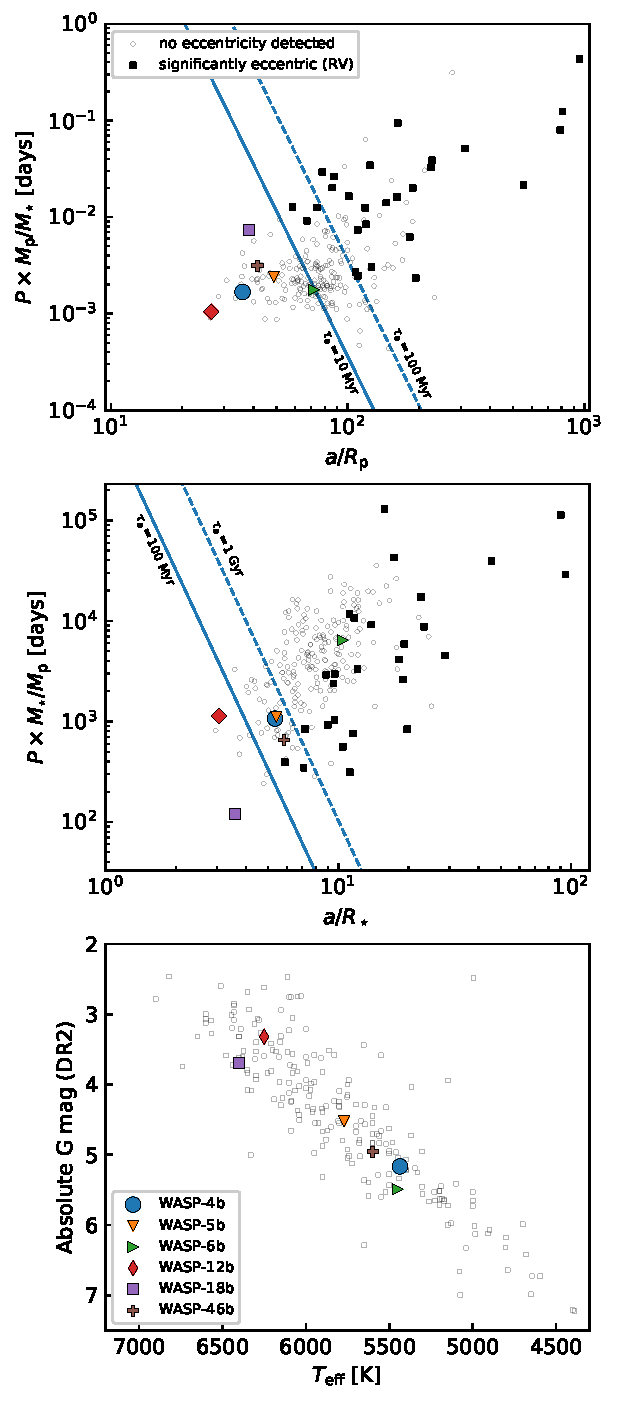
\includegraphics[width=0.38\textwidth]{f5.pdf}
  \end{center}
  \vspace{-0.5cm}
  \caption{
    {\bf WASP-4b in the context of other hot Jupiters.}
    Most of the data in these plots are from \citet{bonomo_gaps_2017},
    who measured the eccentricities using radial velocities.  The
    colored symbols highlight WASP-4, WASP-12 (which also shows
    evidence for a decreasing period), and the collection of hot
    Jupiters analyzed in Appendix A.
    {\bf \it Top:}
    The key parameters relevant to eccentricity damping.  Solid
    squares represent planets with a securely detected nonzero
    eccentricity. Lines of constant damping timescale are drawn based
    on Equation~\ref{eq:de_dt} and assuming $Q_{\rm p}' = 10^5$.
    WASP-4b has one of the shortest eccentricity damping timescales.
    {\bf \it Middle:} 
    Plotted are the key parameters relevant to orbital decay.  Lines
    of constant decay timescale are drawn based on
    Equation~\ref{eq:da_dt}), assuming $Q_\star' = 10^7$.  WASP-4b has
    a relatively short orbital decay timescale, although it is not as
    extreme a case in this regard as it is for eccentricity damping.
    {\bf \it Bottom:}
    A Hertzsprung-Russell diagram for hot Jupiter hosts. WASP-4
    appears to be on the main sequence.
    \label{fig:context}
  }
\end{figure}

\subsection{Orbital decay}

If the timing variation is being caused caused entirely by orbital
decay, then the characteristic timescale of the decay is
\begin{equation}
  \frac{P}{ \dot{P} } = 9.2 \, {\rm Myr}.
\end{equation}
For comparison, the corresponding time for WASP-12b is 3.2\,Myr
\citep{patra_2017}.

If WASP-4 really is undergoing rapid orbital decay, then how many of
the other known hot Jupiters should have orbits that are decaying at
detectable (or nearly detectable) rates?  Figure~\ref{fig:context}
compares some key properties of WASP-4 with those of a larger ensemble
of hot Jupiters.  The middle panel displays two parameters that
strongly affect the expected orbital decay timescale, $P
M_\star/M_{\rm p}$ and $a/R_\star$.  WASP-4 has one of the shortest
theoretical timescales for orbital decay.  There are about 20 hot
Jupiters (including WASP-12) for which the theoretical timescale is
shorter.  In almost all of those cases, though, the planet was
discovered more recently than WASP-4 and a decade-long baseline of
observations is not yet available.  A separate consideration not shown
in Figure~\ref{fig:context} is that the hot Jupiter host stars have a
variety of different structures, from being fully convective to nearly
fully radiative, which may lead to widely divergent tidal dissipation
timescales.

In the simple ``constant phase lag'' model for tidal interaction
\citep{zahn_tidal_1977}, the rate of dissipation can be parametrized
by a modified\footnote{For stars, $k_\star \sim \mathcal{O}(10^{-2})$,
  so it is important to explicitly distinguish $Q_\star'$ from
  $Q_\star$ \citep[{\it e.g.},][]{schwarzschild_structure_1958}.}
quality factor, $Q_\star' = 3 Q_\star / (2k_\star)$.
Here, $Q_\star$ is the ratio between the energy stored in the
equilibrium deformation of the star and the energy lost to heat per
tidal period \citep[{\it e.g.},][]{goldreich_q_1966}.  A larger
$Q_\star$ implies less efficient tidal dissipiation. The dimensionless
number $k_\star$ is the stellar Love number, which is smaller when the
star's density distribution is more centrally concentrated.  In this
model, once the planet's spin and orbit are synchronized, then the
semi-major axis and eccentricity evolve as \citep[Appendix B
of][]{metzger_optical_2012}
\begin{align}
  \frac{1}{\tau_{\rm e}} &=
  \frac{|\dot{e}|}{e} =
    \frac{63 \pi } {2 Q_{\rm p}' }
    \left( \frac{R_{\rm p}}{a} \right)^5
    \left( \frac{M_\star}{M_{\rm p}} \right)
    \left( \frac{1}{P} \right)
  \label{eq:de_dt}
  \\
  \frac{1}{\tau_{\rm a}} &=
  \frac{|\dot{a}|}{a} =
    \frac{9 \pi } {Q_\star' }
    \left( \frac{R_\star}{a} \right)^5
    \left( \frac{M_{\rm p}}{M_\star} \right)
    \left( \frac{1}{P} \right).
  \label{eq:da_dt}
\end{align}
The orbital period evolves as
\begin{equation}
\label{eq:dP_dt}
  \dot{P} = -\frac{27\pi}{2 Q_\star'}
            \left(\frac{M_{\rm p}}{M_\star}\right)
            \left(\frac{R_\star}{a}\right)^5.
\end{equation}
The modified quality factor of WASP-4 corresponding to the observed
value of $\dot{P}$ is
\begin{equation}
	Q_\star' \approx 2.9\times10^4.
\end{equation}
This is about an order of magnitude lower than the value that was
inferred for WASP-12b.  It is also smaller than most theoreticians
would have expected.  The $Q_{\rm Jup}'$ value of Jupiter is estimated
to be $\approx$$1.4 \times 10^5$, based on the observed motions of the
Galilean moons \citep{lainey_strong_2009}.  For stars, studies of the
binary eccentricity distribution have been interpreted with tidal
models, giving $Q_\star' \approx 10^5 - 10^7$ \citep[{\it
    e.g.},][]{meibom_robust_2005,belczynski_compact_2008,
  geller_direct_2013,milliman_wiyn_2014}.  Population studies of hot
Jupiter systems have also been undertaken, generally finding $Q_\star'
\approx 10^5 - 10^8$ using different models
\citep{jackson_observational_2009,hansen_calibration_2010,penev_constraining_2012,penev_empirical_2018,cameron_hierarchical_2018}.
For instance, motivated by the rapid rotation of some hot Jupiter
hosts
\citep{pont_empirical_2009,ciceri_hats-15b_2016,penev_hats-18b_2016},
\citet{penev_empirical_2018} modeled the evolution of hot Jupiter
systems under the influence of a magnetized wind and a constant
phase-lag tide.  For WASP-4, their method gave $Q_\star' \approx
(1.2^{+1.0}_{-0.5})\times10^7$.  This strongly disagrees with the
quality factor we have inferred from the apparent period change.

\citet{essick_orbital_2016} studied the problem of the orbital decay
of hot Jupiters using a theory in which gravity modes are excited at
the base of the stellar convective zone, propagate inward through the
radiative core and break near the stellar core, leading to energy
dissipation.  They predicted the stellar quality factors in hot
Jupiter systems to vary from $Q_\star' \approx 10^5 - 10^6$.  From
their Equation 26, the prediction for WASP-4 is $Q_\star' =
7\times10^5$, which is an order of of magnitude larger than implied by
the observed period change.

The applicability of the \citet{essick_orbital_2016} model depends on
the evolutionary state of the star. \citet{weinberg_tidal_2017} showed
that more rapid dissipation --- enough to account for the period
change of WASP-12b --- could exist in stars that have begun evolving
into red giants.  The bottom panel of Figure~\ref{fig:context} shows a
Hertzsprung-Russell diagram of hot Jupiters hosts, including WASP-4.
On the y-axis is $G=g-\mu$, for $g$ the apparent Gaia-band magnitude,
and $\mu$ the distance modulus reported by
\citet{gaia_collaboration_gaia_2018}.  The x-axis is the effective
temperature from \citet{bonomo_gaps_2017}, which for WASP-4 agrees
within $1\sigma$ of that from Table~1.  Inspecting the HR diagram,
WASP-4 shows little evidence of being evolved, in agreement with our
analysis from \S~\ref{sec:system_parameters}.
%%%%%%%%%%%%%%%%%%%%%%%%%%%%%%%%%%%%%%%%%%
% By a similar argument though, WASP-12 would not clearly stand out as a
% candidate subgiant, and \citet{weinberg_tidal_2017} suggest it may in
% fact be a subgiant (though \citealt{bailey_understanding_2019} do not
% find evidence that supports this suggestion).  A more thorough
% isochronal analysis would be of interest, particularly if the transit
% and occultation times continue to vary.  Such an analysis is beyond
% the scope of this study.
%%%%%%%%%%%%%%%%%%%%%%%%%%%%%%%%%%%%%%%%%%

To summarize, if the observed period change is caused entirely by
tidal orbital decay, then the constant-phase-lag tidal model implies a
stellar tidal dissipation rate that is higher than expected by at
least an order of magnitude.  It might be possible that we are
observing at a special time, shortly after the planet's inward
migration, or when the planet is near resonance with a stellar
oscillation mode.  Tidal dissipation rates might also be increased if
the star is just turning off the main sequence.  Another hypothesis,
recently advanced by \citet{millholland_obliquity_2018} for the case
of WASP-12b, is that an exterior planet could be trapping WASP-4b's
spin vector in a high-obliquity state, leading to rapid dissipation
through planetary obliquity tides.

\subsection{Apsidal precession}
\label{sec:apsidal_precession}

If instead the observed timing variation is just a small portion of an
apsidal precession cycle, then the orbital eccentricity is a few times
$10^{-3}$, and the full precession period is about 24 years.
\citet{ragozzine_probing_2009} calculated apsidal precession periods
for hot Jupiters, finding them to range between about 10 and 100
years. They highlighted that for many hot Jupiters, including WASP-4b,
the theoretical precession rate is dominated by the non-Keplerian
force due to the planet's tidal bulge.  Precession from general
relativity, the planet's rotational bulge, and the star's rotational
and tidal bulges contribute at the 10\% level at most.  Thus, a
measurement of the precession rate can be used to determine the
planet's Love number.  From their Equation 14, the implied Love number
for WASP-4b is
\begin{equation}
k_{2,{\rm p}} = 1.5^{+2.1}_{-1.1}.
\end{equation}
For comparison, the Love number of Jupiter is about 0.55
\citep{wahl_tidal_2016,ni_empirical_2018}, and a uniform density
sphere has $k_2 = 1.5$. The uncertainty in $k_{2,{\rm p}}$ for WASP-4b
is large because the eccentricity, reference time, and ${\rm
d}\omega/{\rm d}E$ have strongly correlated errors, and the measured
occultation times only barely constrain these parameters
(Figure~\ref{fig:future}).

The main problem with the apsidal precession hypothesis is to explain
why the eccentricity would be as large as $\sim$$10^{-3}$ despite
rapid tidal circularization.  For WASP-4, Equation~\ref{eq:de_dt}
gives $\tau_e = 0.30 (Q_{\rm p}'/10^5) \, {\rm Myr}$.  The star is
several billion years old, so unless the planet arrived very recently,
any initial eccentricity should have been lowered well below
$\sim$$10^{-3}$.  The top panel of Figure~\ref{fig:context} compares
the expected eccentricity damping time of WASP-4b with that of other
transiting giant planets.  WASP-4b has one of the shortest known
eccentricity damping times.

\paragraph{Neighboring companion}
One way to maintain a significant eccentricity is through the
gravitational perturbations from another planet.
\citet{mardling_long-term_2007} considered the long-term tidal
evolution of hot Jupiters with companions.  The companion in their
model is coplanar, and can have a mass down to an Earth-mass; the main
requirement is that both the hot Jupiter and the outer companion start
on eccentric orbits.  They found that although the early phases of the
two-planet eccentricity evolution occur quickly, the final phase of
the joint eccentricity evolution towards circularity would occur on
timescales several orders of magnitude longer than the circularization
time of an isolated hot Jupiter (see their Figures~4 and 5).
 
A different way to excite the hot Jupiter's eccentricity is the
Kozai-Lidov mechanism \citep{lidov_evolution_1962,kozai_secular_1962}.
In this case, the orbital plane of the outer companion, ``c'', would
need to be inclined relative to that of the hot Jupiter, ``b'', by at
least $\sin^{-1} \sqrt{2/5} \approx 39^\circ$.
For the Kozai-Lidov mechanism to operate at maximum efficiency, we
need \citep[][Equation 20]{bailey_understanding_2019}
\begin{equation}
  M_{\rm c} > 7.1\,M_\oplus
  \times \left( \frac{a_{\rm c}}{a_{\rm b}} \right)^{3/2},
  \label{eq:kozai_bound}
\end{equation}
where $M_{\rm b,c}$ and $a_{\rm b,c}$ are the mass and semi-major axis
of WASP-4b and the hypothetical WASP-4c, and we have assumed WASP-4b's
Love number is $k_{2,{\rm b}}\approx 0.6$.  For the RV signal of the
companion to remain undetected, it would need to be in the residual
$({\rm O-C})_{\rm RV} = 15.2\,{\rm m s}^{-1}$ reported by
\citet{triaud_spin-orbit_2010}.  Again following
\citet{bailey_understanding_2019}, this implies
\begin{align}
  M_{\rm c} &<
  ({\rm O-C})_{\rm RV}
  \left( \frac{M_\star a_b}{G} \right)^{1/2}
  \left( \frac{a_c}{a_b} \right)^{1/2}
  f^{-1/2}
  \nonumber
  \\
  M_{\rm c} &< 
  23.8\,M_\oplus
  \times 
  \left( \frac{a_c}{a_b} \right)^{1/2}
  f^{-1/2},
  \label{eq:rv_bound}
\end{align}
for $f(e_{\rm c},\omega_{\rm c}, i_{\rm c}) \propto \sin^2 i_{\rm c}$
a geometric prefactor that depends on the argument of periastron
$\omega_{\rm c}$ and inclination $i_{\rm c}$ of the exterior companion
(\citealt{bailey_understanding_2019} Equation 23).  Since WASP-4b is
transiting, $f$ can be arbitrarily small, and both of the preceding
limits can be satisfied. 

\paragraph{Fluctuations in the gravitational potential from convection}
A separate mechanism to pump the eccentricity invokes the
gravitational fluctuations from stellar convection \citep[][Section
7]{phinney_pulsars_1992}.  From equation 7.33 of that work, the
mean-squared eccentricity of the orbit is
\begin{equation}
  \langle e^2 \rangle =
  \frac{ 2 \langle E_{\rm e} \rangle }{\mu n^2 a^2}
  = 6.8\times10^{-5}
  \frac{(L^2 R_{\rm conv}^2 M_{\rm conv}^2)^{1/3}}{\mu n^2 a^2},
\end{equation}
where $L$ is the stellar luminosity, $R_{\rm conv}$ and $M_{\rm conv}$
are the width and mass of the convective region, $\mu$ is the reduced
mass, $n$ is the orbital frequency, and $a$ is the semi-major axis.
For WASP-4, this equation implies $\langle e^2 \rangle^{1/2} \lesssim
10^{-5}$.  Hence, this mechanism does not seem capable of producing
the required value of $\sim$$10^{-3}$.

%%%%%%%%%%%%%%%%%%%%%%%%%%%%%%%%%%%%%%%%%%
% LB: I calculated the above using MESA grids from Penev+ 2018 to
% estimate the core/envelope masses, but mentioning this is too
% detailed.
%%%%%%%%%%%%%%%%%%%%%%%%%%%%%%%%%%%%%%%%%%

\subsection{Applegate effect}

Some eclipsing binaries exhibit period modulations with amplitudes of
$\lesssim 0.05\,{\rm days}$ over timescales of decades \citep[{\it
    e.g.},][]{soderhjelm_geometry_1980,hall_relation_1989}.
\citet{applegate_mechanism_1992} proposed a mechanism to explain these
modulations in which the internal structure of a magnetically active
star changes shape via cyclic exchange of angular momentum between the
inner and outer zones of the star.  This model could also apply to a
hot Jupiter orbiting a star with a convective zone.  The changing
gravitational quadrupole of the star would cause the orbit of the
planet to precess on the timescale of the stellar activity cycle.  An
essential difference between this process and apsidal precession is
that Applegate timing variations need not be strictly periodic
\citep[{\it e.g.},][Figure~12]{soderhjelm_geometry_1980}. This
mechanism would also produce transit and occultation timing deviations
of the same sign, while for apsidal precession they would have
opposite signs.  For WASP-4, \citet{watson_orbital_2010} estimated
that the Applegate effect could produce timing deviations of up to 15
seconds, depending on the modulation period of the stellar dynamo, and
the corresponding level of differential surface shear.  If this
analysis is accurate, then the Applegate mechanism cannot explain the
majority our observed $82$ second variation.

\subsection{Other possible explanations}

An apparent change in orbital period can also be caused by an overall
acceleration of the center of mass of the system.  This would produce
a period derivative
\begin{equation}
	\dot{P} \approx \frac{\dot{v}_{\rm r} P}{c},
\end{equation}
where $\dot{v}_{\rm r}$ is the time derivative of the radial velocity.
\citet{knutson_friends_2014} combined radial-velocity data from their
own program as well as those of \citet{wilson_wasp-4b_2008},
\citet{pont_determining_2011}, and \citet{husnoo_observational_2012}
to obtain a constraint on any long-term trend:
\begin{equation}
\dot{v}_{\rm r} =
   -0.0099^{+0.0052}_{-0.0054}
   \,{\rm m}\,{\rm s}^{-1}\,{\rm day}^{-1},
\end{equation}
which can also be expressed as a 2$\sigma$ upper limit of $0.021
\,{\rm m}\,{\rm s}^{-1}\,{\rm day}^{-1}$ on the acceleration along the
line of sight.  The associated upper limit on the apparent period
change resulting from this acceleration is $9\times 10^{-11}$, which
is only one-quarter of the observed period decrease
(Equation~\ref{eq:dP_dt_obs}).

Thus, it seems that the observed period decrease cannot be fully
explained as a constant acceleration of the center of mass of WASP-4.
Given the limited amount and uneven time coverage of the existing
radial-velocity data, it remains possible that the center of mass has
a more complex motion, due to a companion on a highly eccentric orbit
\citep[similar to {\it e.g.}, WASP-53 or WASP-81][]{triaud_peculiar_2017}.
It would be useful to gather more radial-velocity data to confirm or
refute this possibility.

There are two other small effects worth noting.  The first is the
\citet{shklovskii_possible_1970} effect due to the star's proper
motion, which leads to an apparent period change of $P\mu^2 d/ c$,
which is only $6\times10^{-13}$ for the case of WASP-4.  The second
effect, described by \citet{rafikov_stellar_2009}, comes from the
star's on-sky motion altering our viewing angle, and leads to an
observed apsidal precession. The corresponding period change is
$\dot{P} \sim (P\mu)^2/2\pi$, which is on the order of $10^{-21}$ for
WASP-4, too small to be of any consequence.


%%%%%%%%%%%%%%%%%%%%%%%%%%%%%%%%%%%%%%%%%%
\section{Call for additional observations}
\label{sec:future}

\begin{figure}[t]
	\begin{center}
		\leavevmode
		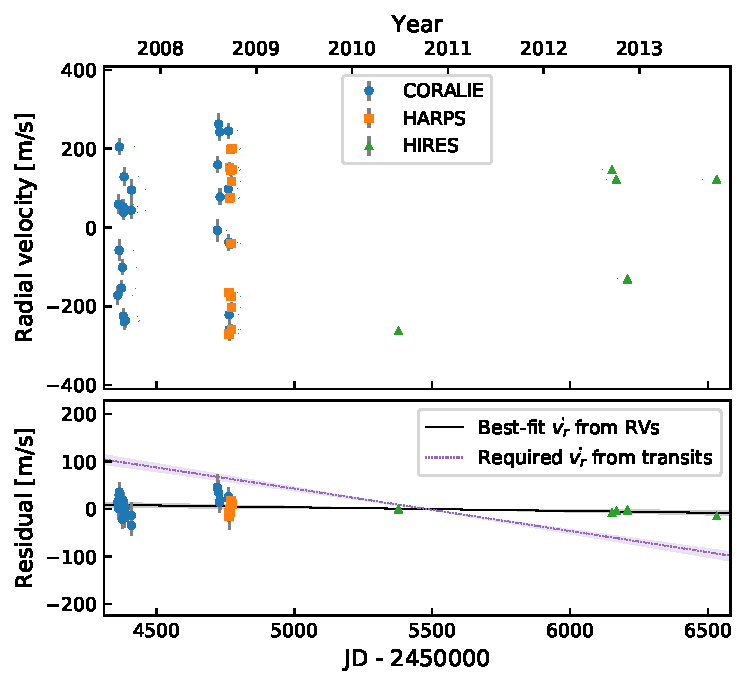
\includegraphics[width=0.49\textwidth]{f6.pdf}
	\end{center}
	\vspace{-0.5cm}
	\caption{
    {\bf Further observations will be needed to confirm and understand
    the timing variations of WASP-4b.} Dots are as in
    Figure~\ref{fig:times}.  Lines are 100 random draws from the
    posteriors of the apsidal precession model (orange), and the
    orbital decay model (blue).    
		\label{fig:future}
	}
\end{figure}

A primary purpose of this work has been to call attention to the
timing anomaly of WASP-4 that has been sighted by TESS, and alert
observers to the need for follow-up transit timing, occultation
timing, and radial-velocity monitoring.  There is no unique
interpretation of the current data, and two of the possibilities ---
orbital decay and apsidal precession --- would be of great interest to
confirm. Detection of orbital decay would lead to an unusually direct
determination of a stellar dissipation rate. Detection of apsidal
precession would give a rare constraint on the interior density
distribution of an exoplanet.

If the TESS mission is extended after its primary mission, it will
likely observe additional transits of WASP-4b in the early 2020s
(Figure~\ref{fig:future}).  High-precision transit observations with
larger telescopes would also be useful.  In order to decide between
orbital decay and apsidal precession, occultation measurements in both
the near term and also in the mid-2020s will be needed.  More
radial-velocity data would help in the search for additional bodies
that could be causing dynamical perturbations, or an overall acceleration
of the host star.

TESS will also be monitoring the other known hot Jupiters, which will
reveal whether the timing anomalies seen in WASP-12 and now WASP-4 are
commonplace, and may shed some light on the circumstances in which
they arise. Other wide-field photometric surveys, such as the Next
Generation Transit Survey \citep{wheatley_next_2018}, HATPI
(\href{https://hatpi.org}{hatpi.org}) and
PLATO \citep{rauer_plato_2014} will also extend
the time baseline of transit timing for a large number of systems.

\acknowledgements
L.G.B.\ gladly acknowledges helpful discussions with
A.~Bailey, F.~Dai and V.~Van Eylen, and is grateful to the
people who have turned TESS from an idea into reality.
%
J.N.W.\ thanks the TESS project and the Heising-Simons foundation for
supporting this work.
%
WASP-4 was included on the ``short-cadence'' target list thanks to the
Guest Investigator programs of J.\ Southworth and S.\ Kane (G011112
and G011183 respectively). 
%
This paper includes data collected by the TESS mission, which are
publicly available from the Mikulski Archive for Space Telescopes
(MAST).
%
Funding for the TESS mission is provided by NASA's Science Mission
directorate.
%
This research has made use of the NASA Exoplanet Archive, which is
operated by the California Institute of Technology, under contract
with the National Aeronautics and Space Administration under the
Exoplanet Exploration Program.
%
This work made use of NASA's Astrophysics Data System Bibliographic
Services.
%
This research has made use of the VizieR catalogue access tool, CDS,
Strasbourg, France. The original description of the VizieR service was
published in A\&AS 143, 23.
%
This work has made use of data from the European Space Agency (ESA)
mission {\it Gaia} (\url{https://www.cosmos.esa.int/gaia}), processed
by the {\it Gaia} Data Processing and Analysis Consortium (DPAC,
\url{https://www.cosmos.esa.int/web/gaia/dpac/consortium}). Funding
for the DPAC has been provided by national institutions, in particular
the institutions participating in the {\it Gaia} Multilateral
Agreement.
%
\newline
%
\facility{
	TESS \citep{ricker_transiting_2015},
	Gaia \citep{gaia_collaboration_gaia_2016,gaia_collaboration_gaia_2018}
}
%
\software{
  \texttt{astrobase} \citep{bhatti_astrobase_2018},
  \texttt{astropy} \citep{the_astropy_collaboration_astropy_2018},
  \texttt{astroquery} \citep{astroquery_2018},
  \texttt{BATMAN} \citep{kreidberg_batman_2015},
  \texttt{corner} \citep{corner_2016},
  \texttt{emcee} \citep{foreman-mackey_emcee_2013},
  \texttt{IPython} \citep{perez_2007},
  \texttt{matplotlib} \citep{hunter_matplotlib_2007}, 
  \texttt{numpy} \citep{walt_numpy_2011}, 
  \texttt{pandas} \citep{mckinney-proc-scipy-2010},
  \texttt{scikit-learn} \citep{scikit-learn},
  \texttt{scipy} \citep{jones_scipy_2001}.
}

%\clearpage
%\newpage
%% \begin{deluxetable}{} command tell LaTeX how many columns
%% there are and how to align them.
\startlongtable
\begin{deluxetable}{ccccc}
    
%% Keep a portrait orientation

%% Over-ride the default font size
%% Use Default (12pt)
\tabletypesize{\scriptsize}

%% Use \tablewidth{?pt} to over-ride the default table width.
%% If you are unhappy with the default look at the end of the
%% *.log file to see what the default was set at before adjusting
%% this value.

%% This is the title of the table.
\tablecaption{WASP-4b transit times, uncertainties, and references.}
\label{tab:transit_times}

%% This command over-rides LaTeX's natural table count
%% and replaces it with this number.  LaTeX will increment 
%% all other tables after this table based on this number
\tablenum{1}

%% The \tablehead gives provides the column headers.  It
%% is currently set up so that the column labels are on the
%% top line and the units surrounded by ()s are in the 
%% bottom line.  You may add more header information by writing
%% another line between these lines. For each column that requries
%% extra information be sure to include a \colhead{text} command
%% and remember to end any extra lines with \\ and include the 
%% correct number of &s.
\tablehead{
  \colhead{$t_{\rm tra}$ [BJD$_\mathrm{TDB}$]} &
  \colhead{$\sigma_{t_{\rm tra}}$ [days]} &
  \colhead{Epoch} & 
  \colhead{H13?} & 
  \colhead{Reference}
}

%% All data must appear between the \startdata and \enddata commands
% XXX pasted in from selected_transit_times.tex
\startdata
 2454368.59279 &      0.00033 &   -1059 &       1 &           \citet{wilson_wasp-4b_2008} \\
 2454396.69576 &      0.00012 &   -1038 &       1 &          \citet{gillon_improved_2009} \\
 2454697.79817 &      0.00009 &    -813 &       1 &             \citet{winn_transit_2009} \\
 2454701.81280 &      0.00022 &    -810 &       1 &             \citet{hoyer_tramos_2013} \\
 2454701.81303 &      0.00018 &    -810 &       1 &             \citet{hoyer_tramos_2013} \\
 2454705.82715 &      0.00029 &    -807 &       1 &             \citet{hoyer_tramos_2013} \\
 2454728.57767 &      0.00042 &    -790 &       1 &             \citet{hoyer_tramos_2013} \\
 2454732.59197 &      0.00050 &    -787 &       1 &             \citet{hoyer_tramos_2013} \\
 2454740.62125 &      0.00035 &    -781 &       1 &             \citet{hoyer_tramos_2013} \\
 2454748.65111 &      0.00007 &    -775 &       1 &             \citet{winn_transit_2009} \\
 2454752.66576 &      0.00069 &    -772 &       1 &           \citet{dragomir_terms_2011} \\
 2455041.72377 &      0.00018 &    -556 &       1 &             \citet{hoyer_tramos_2013} \\
 2455045.73853 &      0.00008 &    -553 &       1 &  \citet{sanchis-ojeda_starspots_2011} \\
 2455049.75325 &      0.00007 &    -550 &       1 &  \citet{sanchis-ojeda_starspots_2011} \\
 2455053.76774 &      0.00009 &    -547 &       1 &  \citet{sanchis-ojeda_starspots_2011} \\
 2455069.82661 &      0.00029 &    -535 &       1 &          \citet{nikolov_wasp-4b_2012} \\
 2455069.82670 &      0.00028 &    -535 &       1 &          \citet{nikolov_wasp-4b_2012} \\
 2455069.82617 &      0.00038 &    -535 &       1 &          \citet{nikolov_wasp-4b_2012} \\
 2455069.82676 &      0.00031 &    -535 &       1 &          \citet{nikolov_wasp-4b_2012} \\
 2455073.84128 &      0.00026 &    -532 &       1 &          \citet{nikolov_wasp-4b_2012} \\
 2455073.84108 &      0.00029 &    -532 &       1 &          \citet{nikolov_wasp-4b_2012} \\
 2455073.84111 &      0.00023 &    -532 &       1 &          \citet{nikolov_wasp-4b_2012} \\
 2455073.84114 &      0.00018 &    -532 &       1 &          \citet{nikolov_wasp-4b_2012} \\
 2455096.59148 &      0.00022 &    -515 &       1 &             \citet{hoyer_tramos_2013} \\
 2455100.60595 &      0.00012 &    -512 &       1 &  \citet{sanchis-ojeda_starspots_2011} \\
 2455112.64986 &      0.00039 &    -503 &       1 &          \citet{nikolov_wasp-4b_2012} \\
 2455112.65009 &      0.00033 &    -503 &       1 &          \citet{nikolov_wasp-4b_2012} \\
 2455112.65005 &      0.00031 &    -503 &       1 &          \citet{nikolov_wasp-4b_2012} \\
 2455112.65005 &      0.00049 &    -503 &       1 &          \citet{nikolov_wasp-4b_2012} \\
 2455132.72310 &      0.00041 &    -488 &       1 &             \citet{hoyer_tramos_2013} \\
 2455468.61943 &      0.00046 &    -237 &       1 &             \citet{hoyer_tramos_2013} \\
 2455526.16356 &      0.00008 &    -194 &       0 &       \citet{ranjan_atmospheric_2014} \\
 2455828.60375 &      0.00041 &      32 &       1 &             \citet{hoyer_tramos_2013} \\
 2455832.61815 &      0.00041 &      35 &       1 &             \citet{hoyer_tramos_2013} \\
 2455844.66287 &      0.00009 &      44 &       0 &           \citet{huitson_gemini_2017} \\
 2456216.69123 &      0.00006 &     322 &       0 &           \citet{huitson_gemini_2017} \\
 2456576.67556 &      0.00005 &     591 &       0 &           \citet{huitson_gemini_2017} \\
 2456924.61561 &      0.00006 &     851 &       0 &           \citet{huitson_gemini_2017} \\
 2458355.18490 &      0.00024 &    1920 &       0 &                             This work \\
 2458356.52251 &      0.00026 &    1921 &       0 &                             This work \\
 2458357.86101 &      0.00024 &    1922 &       0 &                             This work \\
 2458359.19951 &      0.00025 &    1923 &       0 &                             This work \\
 2458360.53708 &      0.00027 &    1924 &       0 &                             This work \\
 2458361.87539 &      0.00024 &    1925 &       0 &                             This work \\
 2458363.21412 &      0.00027 &    1926 &       0 &                             This work \\
 2458364.55192 &      0.00025 &    1927 &       0 &                             This work \\
 2458365.89064 &      0.00026 &    1928 &       0 &                             This work \\
 2458369.90503 &      0.00027 &    1931 &       0 &                             This work \\
 2458371.24297 &      0.00026 &    1932 &       0 &                             This work \\
 2458372.58136 &      0.00027 &    1933 &       0 &                             This work \\
 2458373.91982 &      0.00027 &    1934 &       0 &                             This work \\
 2458375.25801 &      0.00024 &    1935 &       0 &                             This work \\
 2458376.59621 &      0.00024 &    1936 &       0 &                             This work \\
 2458377.93443 &      0.00026 &    1937 &       0 &                             This work \\
 2458379.27317 &      0.00026 &    1938 &       0 &                             This work \\
 2458380.61097 &      0.00027 &    1939 &       0 &                             This work \\
\enddata

%% Include any \tablenotetext{key}{text}, \tablerefs{ref list},
%% or \tablecomments{text} between the \enddata and 
%% \end{deluxetable} commands

%% General table comment marker
\tablecomments{
    $t_{\rm tra}$ is the measured transit midtime, and $\sigma_{t_{\rm
    tra}}$ is its $1\sigma$ uncertainty.
    $\sigma_{t_0}$ was evaluated from the sampled posteriors by taking
    the maximum of the difference between the 84th percentile
    minus the median, and the median minus the 16th percentile.
    The ``Reference'' column refers to the work describing the
    original observations.
    The ``H13?'' column is 1 if the mid-time value was taken from 
    \citet{hoyer_tramos_2013}.  Otherwise, the mid-time
    came from the column listed in ``Reference''.
    The \citet{hoyer_tramos_2013} BJD$_{\rm TT}$ times are equal to
    BJD$_{\rm TDB}$ for our purposes \citep{urban_explanatory_2012}.
    We omitted the timing measurements from
    \citet{southworth_high-precision_2009}, since there were technical
    problems with the computer clock at the time of
    observation~\citep{nikolov_wasp-4b_2012}.
}
\end{deluxetable}


%\clearpage
%\newpage
%% \begin{deluxetable}{} command tell LaTeX how many columns
%% there are and how to align them.
\startlongtable
\begin{deluxetable}{cccc}
    
%% Keep a portrait orientation

%% Over-ride the default font size
%% Use Default (12pt)
\tabletypesize{\footnotesize}

%% Use \tablewidth{?pt} to over-ride the default table width.
%% If you are unhappy with the default look at the end of the
%% *.log file to see what the default was set at before adjusting
%% this value.

%% This is the title of the table.
\tablecaption{WASP-4b occultation times, uncertainties, and references.}
\label{tab:occultation_times}

%% This command over-rides LaTeX's natural table count
%% and replaces it with this number.  LaTeX will increment 
%% all other tables after this table based on this number
\tablenum{3}

%% The \tablehead gives provides the column headers.  It
%% is currently set up so that the column labels are on the
%% top line and the units surrounded by ()s are in the 
%% bottom line.  You may add more header information by writing
%% another line between these lines. For each column that requries
%% extra information be sure to include a \colhead{text} command
%% and remember to end any extra lines with \\ and include the 
%% correct number of &s.
\tablehead{
  \colhead{$t_{\rm occ}$ [BJD$_\mathrm{TDB}$]} &
  \colhead{$\sigma_{t_{\rm occ}}$ [days]} &
  \colhead{Epoch} & 
  \colhead{Reference}
}

%% All data must appear between the \startdata and \enddata commands
% XXX pasted in from selected_transit_times.tex
\startdata
 2455102.61210 &      0.00109 &    -511 &  \citet{caceres_ground-based_2011}\tablenotemark{a} \\
 2455172.20159 &      0.00130 &    -459 &      \citet{beerer_secondary_2011} \\
 2455174.87780 &      0.00087 &    -457 &      \citet{beerer_secondary_2011} \\
 2456907.88714 &      0.00290 &     838 &        \citet{zhou_secondary_2015}\tablenotemark{b} \\
\enddata

%% Include any \tablenotetext{key}{text}, \tablerefs{ref list},
%% or \tablecomments{text} between the \enddata and 
%% \end{deluxetable} commands

%% General table comment marker
\tablecomments{
	$t_{\rm occ}$ is the measured occultation midtime, minus the
	$2a/c=22.8$ second light travel time;
	$\sigma_{t_{\rm occ}}$ is the $1\sigma$ uncertainty on the occultation
	time.
}
\tablenotetext{a}{
\citet{caceres_ground-based_2011} reported this time in ``HJD'', with
an unspecified time standard. We assumed the time was originally in
${\rm HJD}_{\rm UTC}$, inflated the uncertainties by 69.184 seconds,
and converted to ${\rm BJD}_{\rm TDB}$ for the time reported.
}
\tablenotetext{b}{
\citet{zhou_secondary_2015} fixed the epoch, and let $e\cos\omega$
float. Using the reported dates of observation, we converted their
$e\cos\omega$ values into an occultation time using
Equation~\ref{eq:occultation_time} of the text. 
}

\end{deluxetable}


%\clearpage
%\newpage
%\renewcommand{\arraystretch}{1.0}

\startlongtable
\begin{deluxetable}{lc}

\tabletypesize{\footnotesize}

\tablenum{4}

%\tablewidth{0pt}

\tablecaption{Best-fit model parameters.}
\label{tab:bestfit}

\tablehead{
  \colhead{Parameter} &
  \colhead{Median Value~(Unc.)\tablenotemark{a}}
}

\startdata
~~~~~~{\it Constant period} &  \\
$t_0$\,[${\rm BJD}_{\rm TBD}$]    & 2455804.515752(+19)(-19)              \\
$P$\,[days]                       & 1.338231466(+23)(-22)                 \\
~~~~~~{\it Constant period derivative} &  \\
$t_0$~[${\rm BJD}_{\rm TBD}$]     & 2455804.515918(+24)(-24)              \\
$P$\,[days]                       & 1.338231679(+31)(-31)                 \\
$dP/dt$                           & $-4.00(+37)(-38) \times 10^{-10}$     \\
~~~~~~{\it Apsidal precession} &  \\
$t_0$~[${\rm BJD}_{\rm TBD}$]     & 2455804.51530(+25)(-31)               \\
$P_{\rm s}$\,[days]               & 1.33823127(+20)(-48)                  \\
$e$                               & $1.92^{+1.93}_{-0.76} \times 10^{-3}$ \\
$\omega_0$\,[rad]                 & 2.40(+38)(-34)                        \\
$d\omega/dE$~[rad\,epoch$^{-1}$]  & $8.70^{+3.01}_{-2.30} \times 10^{-4}$ \\
\enddata
\tablenotetext{a}{
The numbers in parenthesis give the $68\%$ confidence interval for the final
two digits, where appropriate.
}
\end{deluxetable}



\clearpage

\bibliographystyle{yahapj}                            
\bibliography{bibliography} 

%\clearpage
%\newpage

\appendix

%%%%%%%%%%%%%%%%%%%%%%%%%%%%%%%%%%%%%%%%%%
\section{Verifying the TESS Time Stamps}
\label{sec:verify_tess}

An obvious concern that one might have about the WASP-4 timing anomaly
is that there might be a systematic offset between the TESS time
system and the time system in which the previous observations have
been reported.  There is a precedent for this type of error: data from
the Kepler mission was afflicted by a systematic timing error that was
corrected only late in the mission~\citep[][Section
  3.4]{kepler_DR19_2013}. We performed two checks on the calibration
of the TESS time system, described below.

\subsection{Checking for consistency in the headers of the lightcurve files}
\label{sec:headers}

The TESS lightcurve files provide observation start and end times in
three different time systems: ${\rm JD}_{\rm UTC}$, ${\rm JD}_{\rm
TDB}$, and ${\rm BJD}_{\rm TDB}$.  First, we verified for a few select
lightcurve files that ${\rm JD}_{\rm UTC}$ lagged behind ${\rm
JD}_{\rm TDB}$ by the expected $32.184 + N\,{\rm seconds}$, where $N$
is the number of leap-seconds since 1961. For the relevant observation
time, $N=37$, and the offset was as expected.  Then, using the ${\rm
JD}_{\rm UTC}$ timestamp, we calculated the barycentric correction
using the software written by \citealt{eastman_achieving_2010}.  (For
simplicity, we assumed the TESS spacecraft was located at the Earth's
geocenter, because the light-travel time between the geocenter and the
spacecraft is on the order of only one second.)  This gave us times in
${\rm BJD}_{\rm TDB}$ that agreed with the ${\rm BJD}_{\rm TDB}$ times
that are delivered with the TESS data products.

\subsection{Checking for timing anomalies in other hot Jupiter systems}
\label{sec:hj_verification}

\begin{figure*}[ht!]
  \begin{center}
    \leavevmode
    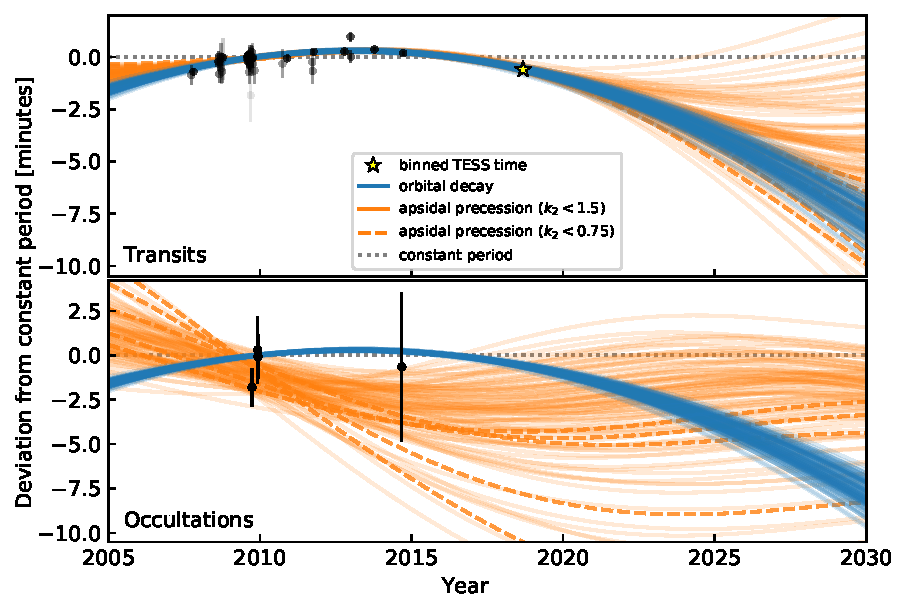
\includegraphics[width=0.9\textwidth]{f7.pdf}
  \end{center}
  \vspace{-0.5cm}
  \caption{
    {\bf There is no evidence for a systematic offset between TESS
    times and the barycentric reference.} While the WASP-4b transits
    fell about 82 seconds earlier than expected, other well-observed
    hot Jupiters, in particular WASP-6b and WASP-18b, arrived on time.
    Ticks are observed TESS transit midtimes; the orange distribution
    is a gaussian centered on zero with standard deviation
    ($\sigma_{\rm predicted}$) calculated from the pre-TESS transit
    times.  The blue distribution is a gaussian centered on the
    weighted average of the TESS times, with width equal to the
    uncertainty in the mean, {\it i.e.}, the standard deviation
    of the TESS residual times divided by $\sqrt{N-1}$, with $N$ the
    number of transits.
    \label{fig:hjs}
  }
\end{figure*}

If the observed timing delay in WASP-4b were caused by a systematic
global offset between the TESS time system and the ${\rm BJD}_{\rm
TDB}$ reference, we would expect that it would be apparent in other
hot Jupiter systems, too. It would also be apparent in eclipsing
binary observations and any other periodic phenomena that have been
observed over a long time baseline. Here we examine only hot Jupiters
because of our greater familiarity with the data.

We repeated all the data reduction and analysis steps described in
this paper for other hot Jupiters observed by TESS for which timing
data exists spanning many years.  First, we checked which hot Jupiters
were observed over the first three TESS sectors using a combination of
\texttt{tessmaps}\footnote{\url{github.com/lgbouma/tessmaps}} and
TEPCat \citep{southworth_homogeneous_2011}.  We then selected hot
Jupiters for which there were at least five distinct epochs reported
in the peer-reviewed literature.  We required that each observation be
of a single transit, that the midpoint be fit as a free parameter, and
that the time system be clearly documented.  Our final hot Jupiter
sample included WASP-4b, 5b, 6b, 18b, and 46b.  The collected and
measured times are given in Tables~5, 6, 7, and 8 for each.

We determined the best-fitting constant-period ephemeris based on the
pre-TESS data. Then we used the parameters and uncertainties in the
best-fitting model to calculate the predicted transit times during
the TESS observation period, as well as the uncertainty in the
predicted times.  The uncertainties are 11, 94, 18, 42, and 59 seconds
for WASP-4b, 5b, 6b, 18b, and 46b, respectively.  By comparing the
observed and predicted times, Figure~\ref{fig:hjs} shows that WASP-4b
is the only hot Jupiter that transited significantly earlier than
expected.

To use these results to place a quantitative limit on any global clock
offset, for each hot Jupiter we considered the model
\begin{equation}
  t_{\rm tra}(E) = t_0 + PE + t_{\rm offset},
\end{equation}
for $t_{\rm offset}$ a systematic constant offset between the reported
timestamps and the true ${\rm BJD}_{\rm TDB}$ reference.  Our priors
were
\begin{align}
  t_0 &\sim \mathcal{N}[t_0', \sigma_{t_0'}], \\
  P &\sim \mathcal{N}[P', \sigma_{P'}], \\
  t_{\rm offset} &\sim \mathcal{U}[-20\sigma_{t_0'},20\sigma_{t_0'}],
\end{align}
where $\mathcal{N}$ and $\mathcal{U}$ denote a normal and uniform
distribution, $(t_0', P')$ are the best-fit reference time and period
using only the pre-TESS transit times, and $(\sigma_{t_0'},
\sigma_{P'})$ are the corresponding uncertainties.

For each planet, we asked: what fraction of the posterior for $t_{\rm
offset}$ is consistent with an offset worse than $81.5$ seconds?  For
WASP-4b, the answer is unsurprisingly 50\%.  For WASP-6b, the most
constraining object, about 1 sample in 2 million is consistent with
such a timing offset ($4.9\sigma$).  For WASP-18b, 1 in 103 samples
would be consistent with this timing offset ($2.3\sigma$), and in
WASP-46b, the limit is 1 in 49 samples ($2.0\sigma$).  For WASP-5b,
the predicted time is too imprecise to rule out timing offsets at the
necessary amplitude.  Multiplying the three independent probabilities
for WASP-5b, 6b, and 18b, we can rule out $t_{\rm offset} < -81.5\
{\rm seconds}$ at $6.4\sigma$, or about about 1 part in 11 billion.

%\clearpage
%\newpage
%% \begin{deluxetable}{} command tell LaTeX how many columns
%% there are and how to align them.
\startlongtable
\begin{deluxetable}{ccccc}
    
%% Keep a portrait orientation

%% Over-ride the default font size
%% Use Default (12pt)
\tabletypesize{\scriptsize}

%% Use \tablewidth{?pt} to over-ride the default table width.
%% If you are unhappy with the default look at the end of the
%% *.log file to see what the default was set at before adjusting
%% this value.

%% This is the title of the table.
\tablecaption{WASP-5b transit times, uncertainties, and references.}
\label{tab:WASP-5b}

%% This command over-rides LaTeX's natural table count
%% and replaces it with this number.  LaTeX will increment 
%% all other tables after this table based on this number
\tablenum{4}

%% The \tablehead gives provides the column headers.  It
%% is currently set up so that the column labels are on the
%% top line and the units surrounded by ()s are in the 
%% bottom line.  You may add more header information by writing
%% another line between these lines. For each column that requries
%% extra information be sure to include a \colhead{text} command
%% and remember to end any extra lines with \\ and include the 
%% correct number of &s.
\tablehead{
  \colhead{$t_{\rm tra}$ [BJD$_\mathrm{TDB}$]} &
  \colhead{$\sigma_{t_{\rm tra}}$ [days]} &
  \colhead{Epoch} & 
  \colhead{Reference}
}

%% All data must appear between the \startdata and \enddata commands
\startdata
 2454383.76750 &      0.00040 &    -885 &           \citet{anderson_wasp-5b_2008} \\
 2454387.02275 &      0.00100 &    -883 &           \citet{anderson_wasp-5b_2008} \\
 2454636.17459 &      0.00082 &    -730 &         \citet{fukui_measurements_2011} \\
 2454699.68303 &      0.00041 &    -691 &              \citet{hoyer_transit_2012} \\
 2454707.82465 &      0.00052 &    -686 &              \citet{hoyer_transit_2012} \\
 2454707.82523 &      0.00025 &    -686 &  \citet{southworth_high-precision_2009} \\
 2454730.62243 &      0.00031 &    -672 &  \citet{southworth_high-precision_2009} \\
 2454730.62301 &      0.00076 &    -672 &              \citet{hoyer_transit_2012} \\
 2454761.56356 &      0.00047 &    -653 &              \citet{hoyer_transit_2012} \\
 2454772.96212 &      0.00075 &    -646 &         \citet{fukui_measurements_2011} \\
 2454774.59093 &      0.00030 &    -645 &              \citet{hoyer_transit_2012} \\
 2454787.61792 &      0.00069 &    -637 &              \citet{hoyer_transit_2012} \\
 2455005.82714 &      0.00036 &    -503 &              \citet{hoyer_transit_2012} \\
 2455049.79540 &      0.00080 &    -476 &              \citet{hoyer_transit_2012} \\
 2455075.84947 &      0.00056 &    -460 &             \citet{dragomir_terms_2011} \\
 2455079.10830 &      0.00079 &    -458 &         \citet{fukui_measurements_2011} \\
 2455110.04607 &      0.00089 &    -439 &         \citet{fukui_measurements_2011} \\
 2455123.07611 &      0.00079 &    -431 &         \citet{fukui_measurements_2011} \\
 2455129.58759 &      0.00043 &    -427 &              \citet{hoyer_transit_2012} \\
 2455364.08150 &      0.00110 &    -283 &         \citet{fukui_measurements_2011} \\
 2455377.10955 &      0.00093 &    -275 &         \citet{fukui_measurements_2011} \\
 2455448.75927 &      0.00110 &    -231 &             \citet{dragomir_terms_2011} \\
 2456150.61479 &      0.00056 &     200 &          \citet{moyano_multi-band_2017} \\
 2456150.61396 &      0.00057 &     200 &          \citet{moyano_multi-band_2017} \\
 2458355.50829 &      0.00083 &    1554 &                               This work \\
 2458357.13741 &      0.00071 &    1555 &                               This work \\
 2458358.76412 &      0.00068 &    1556 &                               This work \\
 2458360.39377 &      0.00070 &    1557 &                               This work \\
 2458362.02273 &      0.00073 &    1558 &                               This work \\
 2458363.64908 &      0.00090 &    1559 &                               This work \\
 2458365.27827 &      0.00071 &    1560 &                               This work \\
 2458366.90627 &      0.00075 &    1561 &                               This work \\
 2458370.16411 &      0.00076 &    1563 &                               This work \\
 2458371.79126 &      0.00071 &    1564 &                               This work \\
 2458373.42123 &      0.00075 &    1565 &                               This work \\
 2458375.04910 &      0.00069 &    1566 &                               This work \\
 2458376.67856 &      0.00074 &    1567 &                               This work \\
 2458378.30530 &      0.00087 &    1568 &                               This work \\
 2458379.93419 &      0.00082 &    1569 &                               This work \\
\enddata

%% Include any \tablenotetext{key}{text}, \tablerefs{ref list},
%% or \tablecomments{text} between the \enddata and 
%% \end{deluxetable} commands

%% General table comment marker
\tablecomments{
    $t_{\rm tra}$ is the measured transit midtime, and $\sigma_{t_{\rm tra}}$ is its
    $1\sigma$ uncertainty.
    The ``Reference'' column refers to the work describing the
    original observations.
    All the literature times except for the two \citet{moyano_multi-band_2017}
    times are from the homogeneous \citet{hoyer_transit_2012} analysis.
}

\end{deluxetable}

%% \begin{deluxetable}{} command tell LaTeX how many columns
%% there are and how to align them.
\startlongtable
\begin{deluxetable}{ccccc}
    
%% Keep a portrait orientation

%% Over-ride the default font size
%% Use Default (12pt)
\tabletypesize{\scriptsize}
%% Use \tablewidth{?pt} to over-ride the default table width.
%% If you are unhappy with the default look at the end of the
%% *.log file to see what the default was set at before adjusting
%% this value.

%% This is the title of the table.
\tablecaption{WASP-6b transit times, uncertainties, and references.}
\label{tab:WASP-6b}

%% This command over-rides LaTeX's natural table count
%% and replaces it with this number.  LaTeX will increment 
%% all other tables after this table based on this number
\tablenum{6}

%% The \tablehead gives provides the column headers.  It
%% is currently set up so that the column labels are on the
%% top line and the units surrounded by ()s are in the 
%% bottom line.  You may add more header information by writing
%% another line between these lines. For each column that requries
%% extra information be sure to include a \colhead{text} command
%% and remember to end any extra lines with \\ and include the 
%% correct number of &s.
\tablehead{
  \colhead{$t_{\rm tra}$ [BJD$_\mathrm{TDB}$]} &
  \colhead{$\sigma_{t_{\rm tra}}$ [days]} &
  \colhead{Epoch} & 
  \colhead{Reference}
}

%% All data must appear between the \startdata and \enddata commands
\startdata
 2454425.02167 &      0.00022 &    -398 &        \citet{gillon_discovery_2009} \\
 2455009.83622 &      0.00021 &    -224 &  \citet{tregloan-reed_transits_2015} \\
 2455046.80720 &      0.00015 &    -213 &  \citet{tregloan-reed_transits_2015} \\
 2455073.69529 &      0.00013 &    -205 &  \citet{tregloan-reed_transits_2015} \\
 2455409.79541 &      0.00010 &    -105 &  \citet{tregloan-reed_transits_2015} \\
 2455446.76621 &      0.00058 &     -94 &          \citet{dragomir_terms_2011} \\
 2455473.65439 &      0.00097 &     -86 &     \citet{jordan_ground-based_2013} \\
 2455846.72540 &      0.00045 &      25 &         \citet{sada_extrasolar_2012} \\
 2456088.71801 &      0.00013 &      97 &             \citet{nikolov_hst_2015} \\
 2456095.43974 &      0.00017 &      99 &             \citet{nikolov_hst_2015} \\
 2456132.41082 &      0.00017 &     110 &             \citet{nikolov_hst_2015} \\
 2458357.39410 &      0.00033 &     772 &                            This work \\
 2458360.75573 &      0.00033 &     773 &                            This work \\
 2458364.11691 &      0.00032 &     774 &                            This work \\
 2458370.83872 &      0.00033 &     776 &                            This work \\
 2458374.19952 &      0.00031 &     777 &                            This work \\
 2458377.56026 &      0.00033 &     778 &                            This work \\
 2458380.92185 &      0.00038 &     779 &                            This work \\
\enddata

%% Include any \tablenotetext{key}{text}, \tablerefs{ref list},
%% or \tablecomments{text} between the \enddata and 
%% \end{deluxetable} commands

%% General table comment marker
\tablecomments{
    $t_{\rm tra}$ is the measured transit midtime, and $\sigma_{t_{\rm tra}}$ is its
    $1\sigma$ uncertainty.
    The ``Reference'' column refers to the work describing the
    original observations.
}

\end{deluxetable}

%% \begin{deluxetable}{} command tell LaTeX how many columns
%% there are and how to align them.
\startlongtable
\begin{deluxetable}{ccccc}
    
%% Keep a portrait orientation

%% Over-ride the default font size
%% Use Default (12pt)
\tabletypesize{\scriptsize}
%% Use \tablewidth{?pt} to over-ride the default table width.
%% If you are unhappy with the default look at the end of the
%% *.log file to see what the default was set at before adjusting
%% this value.

%% This is the title of the table.
\tablecaption{WASP-18b transit times, uncertainties, and references.}
\label{tab:WASP-18b}

%% This command over-rides LaTeX's natural table count
%% and replaces it with this number.  LaTeX will increment 
%% all other tables after this table based on this number
\tablenum{7}

%% The \tablehead gives provides the column headers.  It
%% is currently set up so that the column labels are on the
%% top line and the units surrounded by ()s are in the 
%% bottom line.  You may add more header information by writing
%% another line between these lines. For each column that requries
%% extra information be sure to include a \colhead{text} command
%% and remember to end any extra lines with \\ and include the 
%% correct number of &s.
\tablehead{
  \colhead{$t_{\rm tra}$ [BJD$_\mathrm{TDB}$]} &
  \colhead{$\sigma_{t_{\rm tra}}$ [days]} &
  \colhead{Epoch} & 
  \colhead{Reference}
}

%% All data must appear between the \startdata and \enddata commands
\startdata
 2454221.48163 &      0.00038 &   -3730 &    \citet{hellier_orbital_2009} \\
 2455221.30420 &      0.00010 &   -2668 &     \citet{maxted_spitzer_2013} \\
 2455432.18970 &      0.00010 &   -2444 &     \citet{maxted_spitzer_2013} \\
 2455470.78850 &      0.00040 &   -2403 &     \citet{maxted_spitzer_2013} \\
 2455473.61440 &      0.00090 &   -2400 &     \citet{maxted_spitzer_2013} \\
 2455554.57860 &      0.00050 &   -2314 &     \citet{maxted_spitzer_2013} \\
 2455570.58400 &      0.00048 &   -2297 &     \citet{maxted_spitzer_2013} \\
 2455876.55590 &      0.00130 &   -1972 &     \citet{maxted_spitzer_2013} \\
 2456896.14780 &      0.00080 &    -889 &  \citet{wilkins_searching_2017} \\
 2457255.78320 &      0.00030 &    -507 &  \citet{wilkins_searching_2017} \\
 2457319.80100 &      0.00039 &    -439 &  \citet{wilkins_searching_2017} \\
 2458354.45778 &      0.00015 &     660 &                       This work \\
 2458355.39934 &      0.00015 &     661 &                       This work \\
 2458356.34073 &      0.00016 &     662 &                       This work \\
 2458357.28228 &      0.00017 &     663 &                       This work \\
 2458358.22348 &      0.00017 &     664 &                       This work \\
 2458359.16512 &      0.00016 &     665 &                       This work \\
 2458360.10662 &      0.00016 &     666 &                       This work \\
 2458361.04813 &      0.00017 &     667 &                       This work \\
 2458361.98968 &      0.00016 &     668 &                       This work \\
 2458362.93129 &      0.00016 &     669 &                       This work \\
 2458363.87266 &      0.00018 &     670 &                       This work \\
 2458364.81373 &      0.00016 &     671 &                       This work \\
 2458365.75526 &      0.00017 &     672 &                       This work \\
 2458366.69704 &      0.00019 &     673 &                       This work \\
 2458367.63835 &      0.00187 &     674 &                       This work \\
 2458369.52126 &      0.00017 &     676 &                       This work \\
 2458370.46285 &      0.00017 &     677 &                       This work \\
 2458371.40405 &      0.00016 &     678 &                       This work \\
 2458372.34536 &      0.00017 &     679 &                       This work \\
 2458373.28727 &      0.00017 &     680 &                       This work \\
 2458374.22817 &      0.00016 &     681 &                       This work \\
 2458375.16976 &      0.00016 &     682 &                       This work \\
 2458376.11124 &      0.00017 &     683 &                       This work \\
 2458377.05269 &      0.00016 &     684 &                       This work \\
 2458377.99448 &      0.00017 &     685 &                       This work \\
 2458378.93572 &      0.00016 &     686 &                       This work \\
 2458379.87720 &      0.00016 &     687 &                       This work \\
 2458380.81891 &      0.00017 &     688 &                       This work \\
\enddata

%% Include any \tablenotetext{key}{text}, \tablerefs{ref list},
%% or \tablecomments{text} between the \enddata and 
%% \end{deluxetable} commands

%% General table comment marker
\tablecomments{
    $t_{\rm tra}$ is the measured transit midtime, and $\sigma_{t_{\rm tra}}$ is its
    $1\sigma$ uncertainty.
    The ``Reference'' column refers to the work describing the
    original observations.
    All the literature times are from the homogeneous
    \citet{wilkins_searching_2017} analysis.
}

\end{deluxetable}

%% \begin{deluxetable}{} command tell LaTeX how many columns
%% there are and how to align them.
\startlongtable
\begin{deluxetable}{ccccc}
    
%% Keep a portrait orientation

%% Over-ride the default font size
%% Use Default (12pt)
\tabletypesize{\scriptsize}
%% Use \tablewidth{?pt} to over-ride the default table width.
%% If you are unhappy with the default look at the end of the
%% *.log file to see what the default was set at before adjusting
%% this value.

%% This is the title of the table.
\tablecaption{WASP-46b transit times, uncertainties, and references.}
\label{tab:WASP-46b}

%% This command over-rides LaTeX's natural table count
%% and replaces it with this number.  LaTeX will increment 
%% all other tables after this table based on this number
\tablenum{8}

%% The \tablehead gives provides the column headers.  It
%% is currently set up so that the column labels are on the
%% top line and the units surrounded by ()s are in the 
%% bottom line.  You may add more header information by writing
%% another line between these lines. For each column that requries
%% extra information be sure to include a \colhead{text} command
%% and remember to end any extra lines with \\ and include the 
%% correct number of &s.
\tablehead{
  \colhead{$t_{\rm tra}$ [BJD$_\mathrm{TDB}$]} &
  \colhead{$\sigma_{t_{\rm tra}}$ [days]} &
  \colhead{Epoch} & 
  \colhead{Reference}
}

%% All data must appear between the \startdata and \enddata commands
\startdata
 2455396.60785 &      0.00062 &    -673 &  \citet{anderson_wasp-44b_2012} \\
 2455449.53082 &      0.00026 &    -636 &  \citet{anderson_wasp-44b_2012} \\
 2455722.73178 &      0.00023 &    -445 &    \citet{ciceri_physical_2016} \\
 2455757.06195 &      0.00094 &    -421 &    \citet{petrucci_search_2018} \\
 2455858.61833 &      0.00009 &    -350 &    \citet{ciceri_physical_2016} \\
 2456108.92771 &      0.00094 &    -175 &    \citet{petrucci_search_2018} \\
 2456111.79422 &      0.00016 &    -173 &    \citet{ciceri_physical_2016} \\
 2456111.79413 &      0.00012 &    -173 &    \citet{ciceri_physical_2016} \\
 2456111.79424 &      0.00015 &    -173 &    \citet{ciceri_physical_2016} \\
 2456130.38895 &      0.00042 &    -160 &    \citet{petrucci_search_2018} \\
 2456131.81456 &      0.00112 &    -159 &    \citet{petrucci_search_2018} \\
 2456194.75916 &      0.00027 &    -115 &    \citet{ciceri_physical_2016} \\
 2456217.64127 &      0.00015 &     -99 &    \citet{ciceri_physical_2016} \\
 2456217.64156 &      0.00013 &     -99 &    \citet{ciceri_physical_2016} \\
 2456227.65574 &      0.00060 &     -92 &    \citet{petrucci_search_2018} \\
 2456407.88096 &      0.00015 &      34 &    \citet{ciceri_physical_2016} \\
 2456407.88085 &      0.00018 &      34 &    \citet{ciceri_physical_2016} \\
 2456407.88148 &      0.00028 &      34 &    \citet{ciceri_physical_2016} \\
 2456407.88159 &      0.00043 &      34 &    \citet{ciceri_physical_2016} \\
 2456460.80526 &      0.00017 &      71 &    \citet{ciceri_physical_2016} \\
 2456460.80450 &      0.00024 &      71 &    \citet{ciceri_physical_2016} \\
 2456460.80547 &      0.00064 &      71 &    \citet{ciceri_physical_2016} \\
 2456510.86818 &      0.00060 &     106 &    \citet{petrucci_search_2018} \\
 2456510.86699 &      0.00015 &     106 &    \citet{petrucci_search_2018} \\
 2456516.58667 &      0.00119 &     110 &    \citet{petrucci_search_2018} \\
 2456520.88012 &      0.00064 &     113 &    \citet{petrucci_search_2018} \\
 2456533.75260 &      0.00071 &     122 &    \citet{ciceri_physical_2016} \\
 2456533.75480 &      0.00015 &     122 &    \citet{ciceri_physical_2016} \\
 2456576.66289 &      0.00109 &     152 &    \citet{petrucci_search_2018} \\
 2456589.54197 &      0.00090 &     161 &    \citet{petrucci_search_2018} \\
 2456609.56653 &      0.00043 &     175 &    \citet{petrucci_search_2018} \\
 2456839.85440 &      0.00123 &     336 &    \citet{petrucci_search_2018} \\
 2456862.74085 &      0.00048 &     352 &    \citet{petrucci_search_2018} \\
 2456882.76566 &      0.00073 &     366 &    \citet{petrucci_search_2018} \\
 2456885.62429 &      0.00053 &     368 &    \citet{petrucci_search_2018} \\
 2456915.66040 &      0.00123 &     389 &    \citet{petrucci_search_2018} \\
 2456942.83880 &      0.00078 &     408 &    \citet{petrucci_search_2018} \\
 2456948.56384 &      0.00074 &     412 &    \citet{petrucci_search_2018} \\
 2457274.68458 &      0.00184 &     640 &    \citet{petrucci_search_2018} \\
 2457294.70886 &      0.00140 &     654 &    \citet{petrucci_search_2018} \\
 2457550.74797 &      0.00031 &     833 &    \citet{petrucci_search_2018} \\
 2457593.65692 &      0.00024 &     863 &    \citet{petrucci_search_2018} \\
 2457600.80985 &      0.00039 &     868 &    \citet{petrucci_search_2018} \\
 2457610.82286 &      0.00020 &     875 &    \citet{petrucci_search_2018} \\
 2458326.00972 &      0.00091 &    1375 &                       This work \\
 2458327.43899 &      0.00093 &    1376 &                       This work \\
 2458328.86970 &      0.00094 &    1377 &                       This work \\
 2458330.29965 &      0.00105 &    1378 &                       This work \\
 2458331.73234 &      0.00105 &    1379 &                       This work \\
 2458333.15977 &      0.00086 &    1380 &                       This work \\
 2458334.59230 &      0.00095 &    1381 &                       This work \\
 2458336.02222 &      0.00082 &    1382 &                       This work \\
 2458337.45111 &      0.00099 &    1383 &                       This work \\
 2458340.31143 &      0.00093 &    1385 &                       This work \\
 2458341.74347 &      0.00093 &    1386 &                       This work \\
 2458343.17362 &      0.00093 &    1387 &                       This work \\
 2458344.60303 &      0.00110 &    1388 &                       This work \\
 2458346.03436 &      0.00091 &    1389 &                       This work \\
 2458347.46335 &      0.00168 &    1390 &                       This work \\
 2458348.89621 &      0.00086 &    1391 &                       This work \\
 2458350.32672 &      0.00101 &    1392 &                       This work \\
 2458351.75486 &      0.00103 &    1393 &                       This work \\
\enddata

%% Include any \tablenotetext{key}{text}, \tablerefs{ref list},
%% or \tablecomments{text} between the \enddata and 
%% \end{deluxetable} commands

%% General table comment marker
\tablecomments{
    $t_{\rm tra}$ is the measured transit midtime, and $\sigma_{t_{\rm tra}}$ is its
    $1\sigma$ uncertainty.
    The ``Reference'' column refers to the work describing the
    original observations.
    All the literature times are from the homogeneous
    \citet{petrucci_search_2018} analysis. 14 of the lightcurves
    were acquired by ETD observers \citep[see][]{petrucci_search_2018}.
}

\end{deluxetable}





% \section{Verifying the WASP-4 Archival Times}
% \label{sec:verify_archival_times}
% 
% \begin{figure*}[ht!]
%   \begin{center}
%     \leavevmode
%     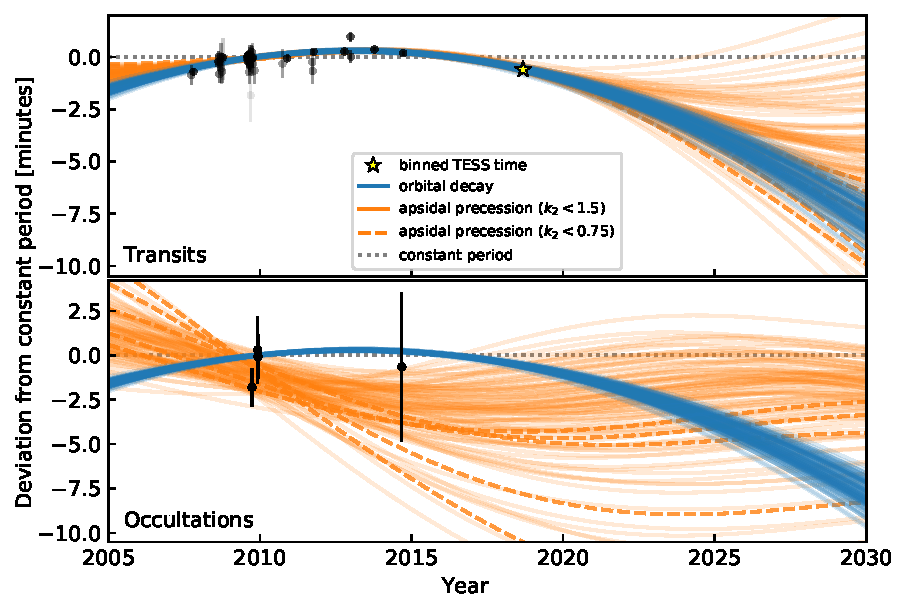
\includegraphics[width=0.9\textwidth]{f7.pdf}
%   \end{center}
%   \caption{
%     {\bf Extra times for WASP-4b neither confirm nor refute the
%     	period-decay.}
%     Our timing analysis (Section~\ref{sec:timing}) imposes stringent
%     selection criteria for lightcurves.
%     Here we overplot additional points from the Exoplanet Transit
%     Database (ETD), and the discovery epoch from \citet{wilson_wasp-4b_2008}.
%     \label{fig:verify}
%   }
% \end{figure*}
% 
% The preceding analysis shows that the TESS timestamps are consistent
% at the requisite level with the ${\rm BJD}_{\rm TDB}$ reference.
% Another explanation for the WASP-4b timing variation could be
% incorrect archival times.
% As a sanity check on the times we included for our analysis in
% Table~1, we collected times from the Exoplanet Transit Database
% \citep[ETD; ][]{poddany_ETD_2010}.  We considered only the 12
% lightcurves of the highest self-reported quality (${\rm DQ} = 1$).  We
% then inspected each lightcurve by eye.  If the lightcurve showed
% substantial red noise, we discarded it.  This left 9 midtimes,
% reported in ${\rm HJD}_{\rm UTC}$. We converted the times to ${\rm
% BJD}_{\rm TDB}$ \citep{eastman_achieving_2010}.
% 
% The resulting times are shown in Figure \ref{fig:verify}.  Focusing on
% the epochs that overlap with \citet{huitson_gemini_2017}'s study, four
% of six possible times agree with the \citet{huitson_gemini_2017}
% times; the other two fall about 90 seconds early.  With their stated
% uncertainties, these 6 ETD data points are inconsistent with a
% constant period.  The 6 points came from 5 different observers.
% Systematic errors in absolute clock offsets by different observers
% should be uncorrelated; if there were such systematic errors in the
% ETD times, this could explain the many-sigma outliers.  Though the
% majority of the reported times do support the accuracy of the
% \citet{huitson_gemini_2017} times, a systematic procedure would call
% for averaging the ETD times.  If we did this, and discarded the four
% \citet{huitson_gemini_2017} epochs, it is likely that the evidence for
% period decay would become much weaker.  Since
% \citet{huitson_gemini_2017} documented their time system clearly, and
% produced lightcurves of extremely high quality, we included their times
% in our analysis.  From private correspondence with
% \citealt{huitson_gemini_2017}, the authors also stand by their
% timestamps. Since the ETD data come from
% heterogeneous sources, their timestamps are less clearly documented,
% and the times are thus more prone to systematic errors, we
% categorically omit them from consideration.
% 
% We also overplotted the discovery epoch reported by
% \citet{wilson_wasp-4b_2008}. 
% This epoch folded together WASP-S survey data, a partial FTS
% lightcurve, and a complete EulerCam lightcurve. 
% Though not explicitly stated by \citet{wilson_wasp-4b_2008}, the
% archival WASP-S lightcurves are in ${\rm HJD}_{\rm UTC}$, so they can
% be converted to ${\rm BJD}_{\rm TDB}$ without uncertainty in the
% absolute time reference (Collier-Cameron, priv.\ comm.).
% The discovery epoch falls about 2 minutes earlier than the epochs we
% used for the fit, and is visible in the lower left of Figure
% \ref{fig:verify}.

% Another independent line of evidence supporting the
% \citet{huitson_gemini_2017} times is that \citet{patra_2017} showed
% for WASP-12b that precise transit times reported by
% \citet{stevenson_transmission_2014} from the Gemini telescopes with
% GMOS are congruent with those from other observers.  This indicates
% that the telescopes do not have a long-standing clock offset.


\end{document}
